%! TEX program = LuaTeX

\documentclass[nobackground,dvipsnames,table,aspectratio=169]{beamer}
\usepackage{cs152}

\mode<presentation>
{\usetheme{Hannover}
    \usecolortheme{cs152}
    \setbeamercovered{transparent}
    \useinnertheme[shadow=false]{rounded}
    \usebackgroundtemplate{}
    \setbeamercolor*{frametitle}{parent=palette primary}
    \setbeamerfont{block title}{size={}}
    \setbeamertemplate{navigation symbols}{}
}

\title{Hate Speech and Incitement}
\subtitle{CS 152 --- Lecture 7}

\author[A. Stamos]{Alex Stamos}
\institute[Stanford University]{Stanford Cyber Policy Center}
\date[2022]{\today}
\subject{CS 152 --- Trust and Safety Engineering}
%\titlegraphic{
\includegraphics[width=5cm]{img/cyber-logo-white-black-red-WEB}}

% Change the level of bulleting on the ToC page
\setcounter{tocdepth}{2}

\graphicspath{{img/lesson07}}

\begin{document}

\begin{frame}
    \titlepage
\end{frame}

\begin{frame}{}
    \thispagestyle{empty}
    \AddToShipoutPictureBG*{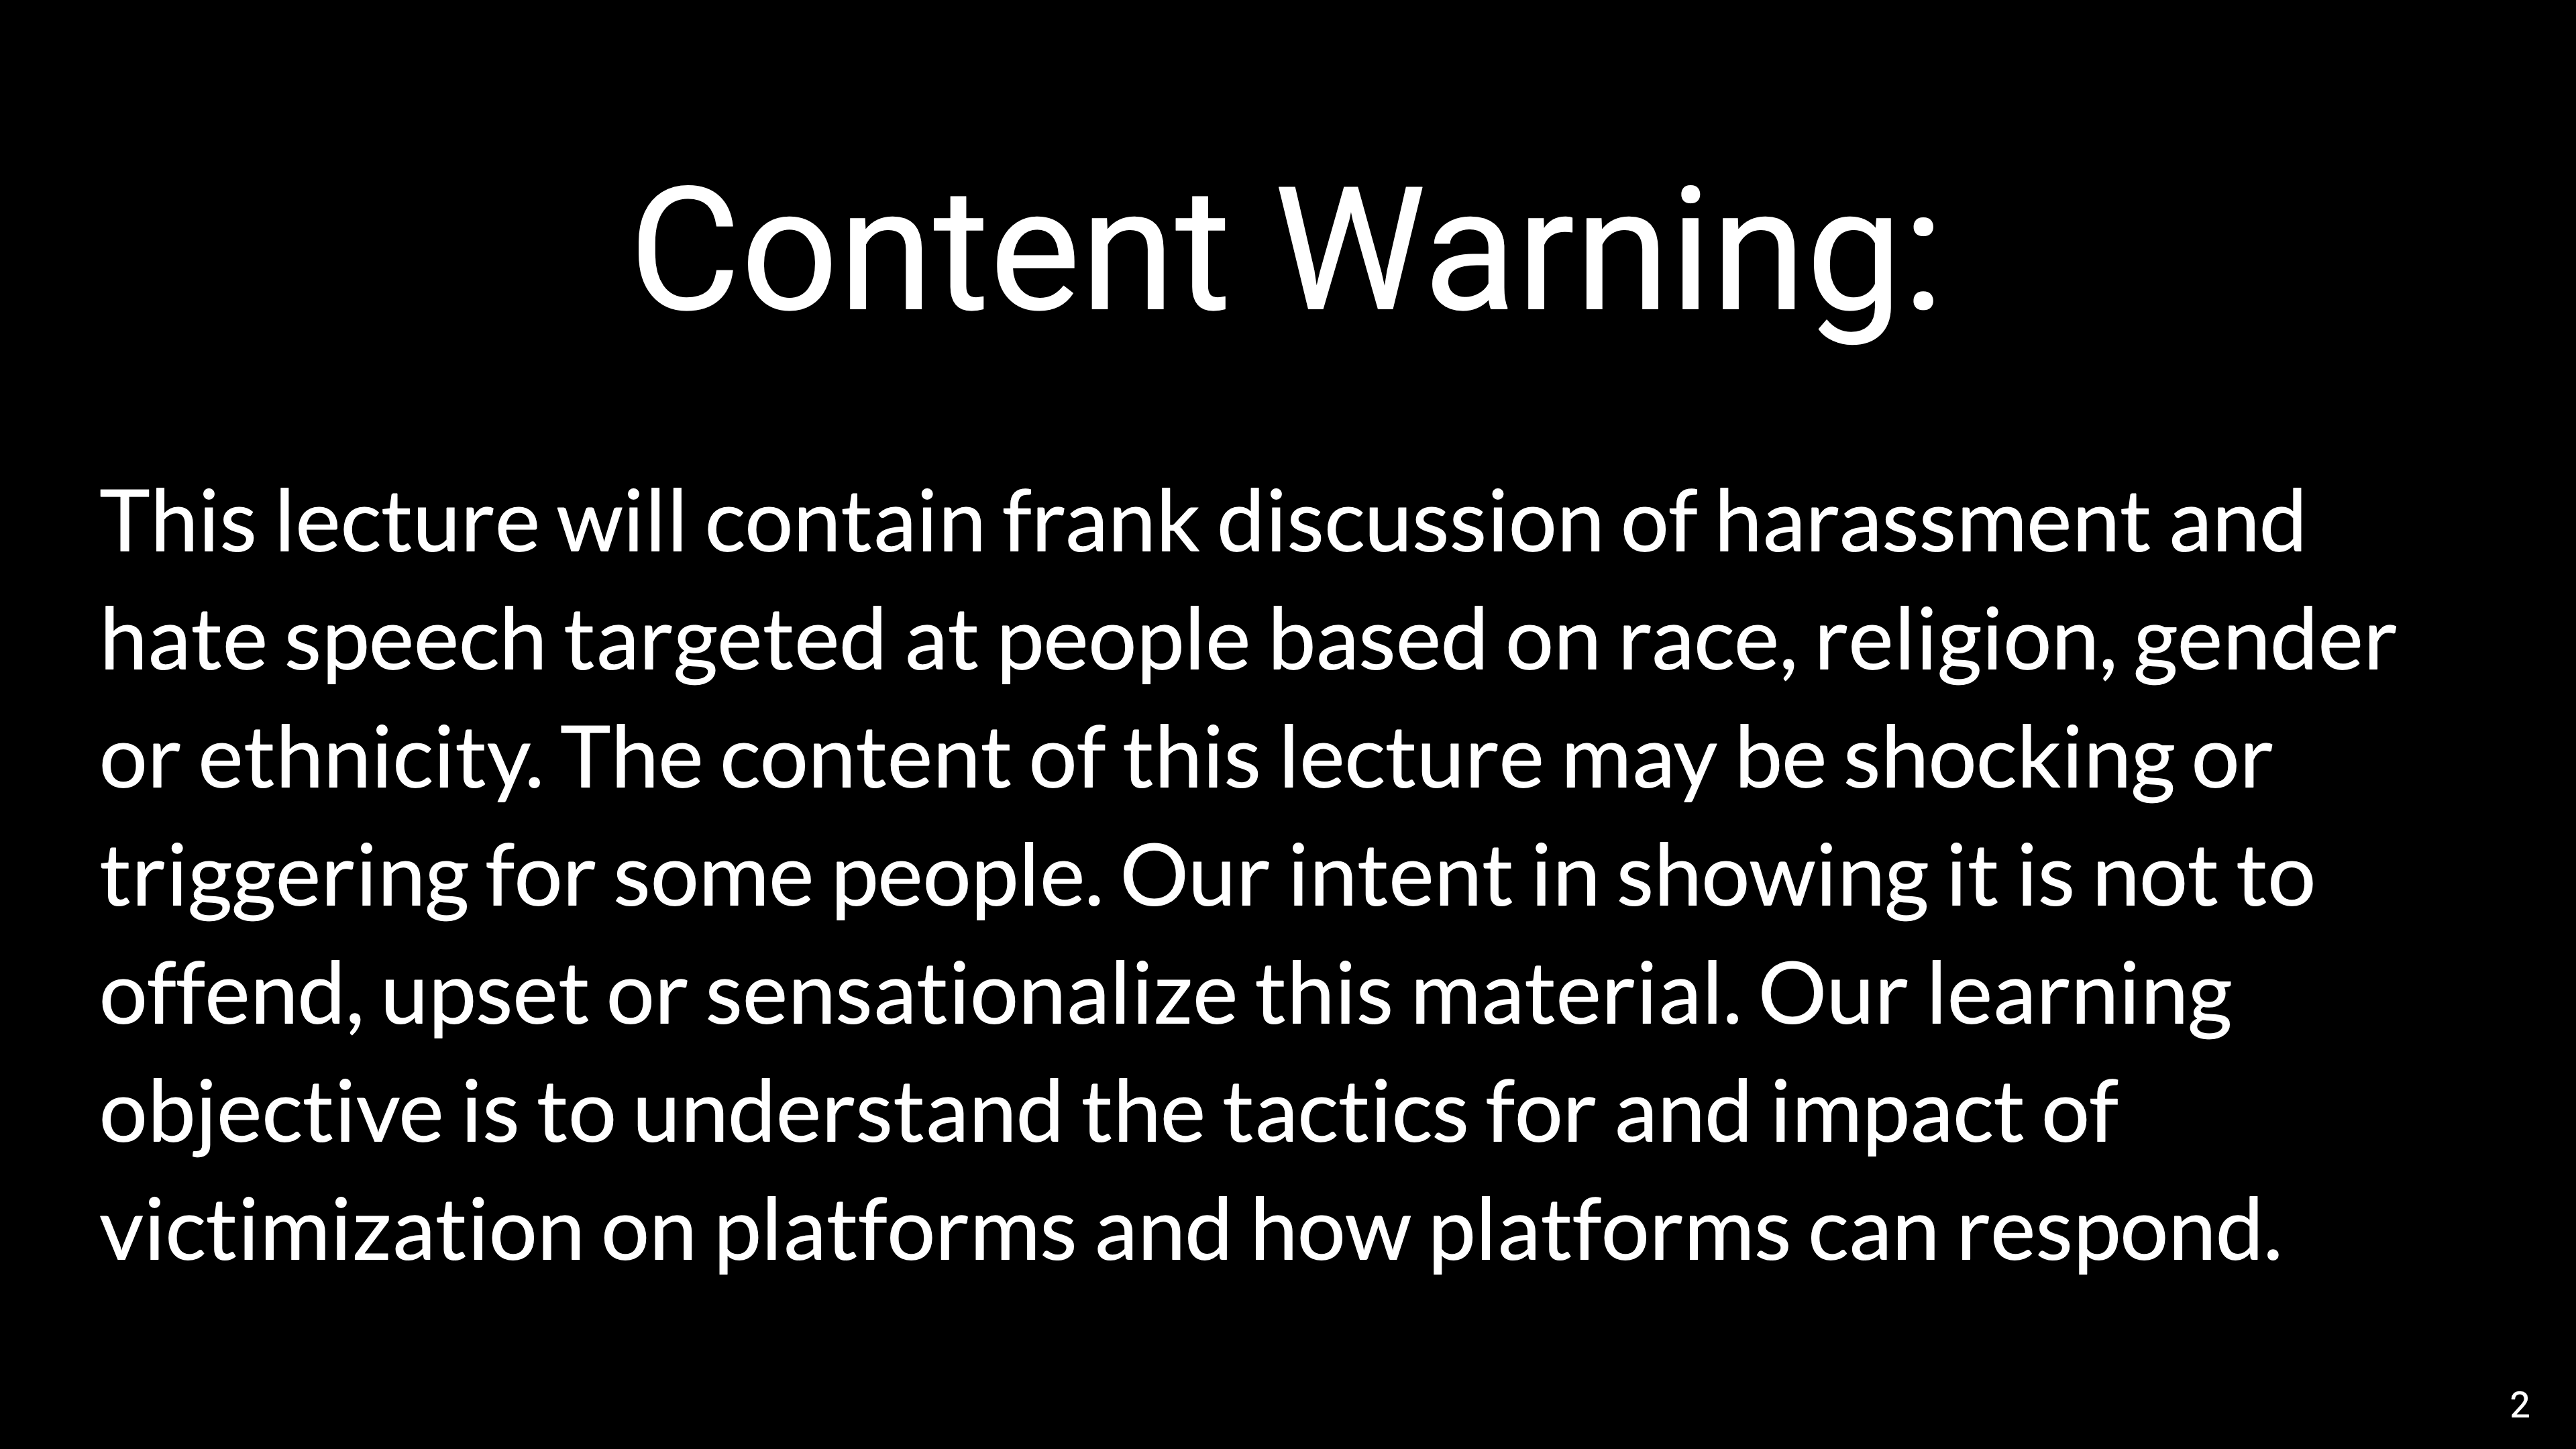
\includegraphics[width=\paperwidth]{content-warning}}
\end{frame}

\begin{frame}{Pepe}
    \begin{columns}
        \column{0.25\textwidth}
            
\includegraphics[width=\textwidth]{pepe}
        \column{0.25\textwidth}
            
\includegraphics[width=\textwidth]{pepe-nazi}
        \column{0.5\textwidth}
            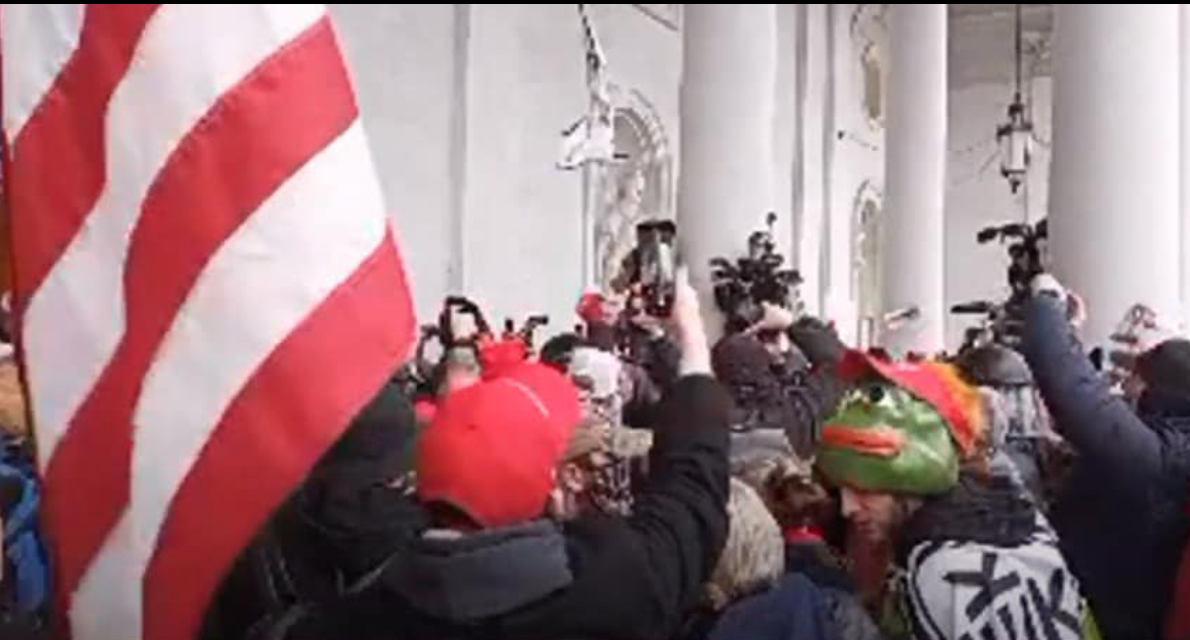
\includegraphics[width=\textwidth]{pepe-jan-6}
    \end{columns}
\end{frame}

\section{What Will You Learn Today?}

\begin{frame}{What Will You Learn Today?}
    \large
    \begin{itemize}
        \item An overview of how hate speech is defined around the world
        \item How quickly hate speech can morph as groups adopt their language to push the same hateful content
        \item Understand the possibilities and limits of AI for hate speech prevention
        \item Review basic platform policies and interventions
    \end{itemize}
\end{frame}

\begin{frame}{Taxonomy}
    \large
    \begin{itemize}
        \item Hate Speech
        \item Hateful Speech
        \item Dangerous Speech
        \item Undesirable Speech
        \item Extremism
    \end{itemize}
\end{frame}

\begin{frame}{Taxonomy}
    If hate speech had a global definition applicable everywhere, it would be easier to tackle it and the field of hate speech would probably be less complex.\\~\\

    However, a single and universal definition is yet to be developed.\\~\\

    Given that, how do we distinguish...\\
    Hate Speech vs. hateful speech?\\
    Hateful Speech vs. cyberharassment?\\
    Dangerous Speech vs. hate speech?\\
    Undesirable Speech vs. hate speech?\\
    Extremism vs. hateful speech?
\end{frame}

\section{Legal Parameters of Hate Speech}

\begin{frame}{}
    \thispagestyle{empty}
    \AddToShipoutPictureBG*{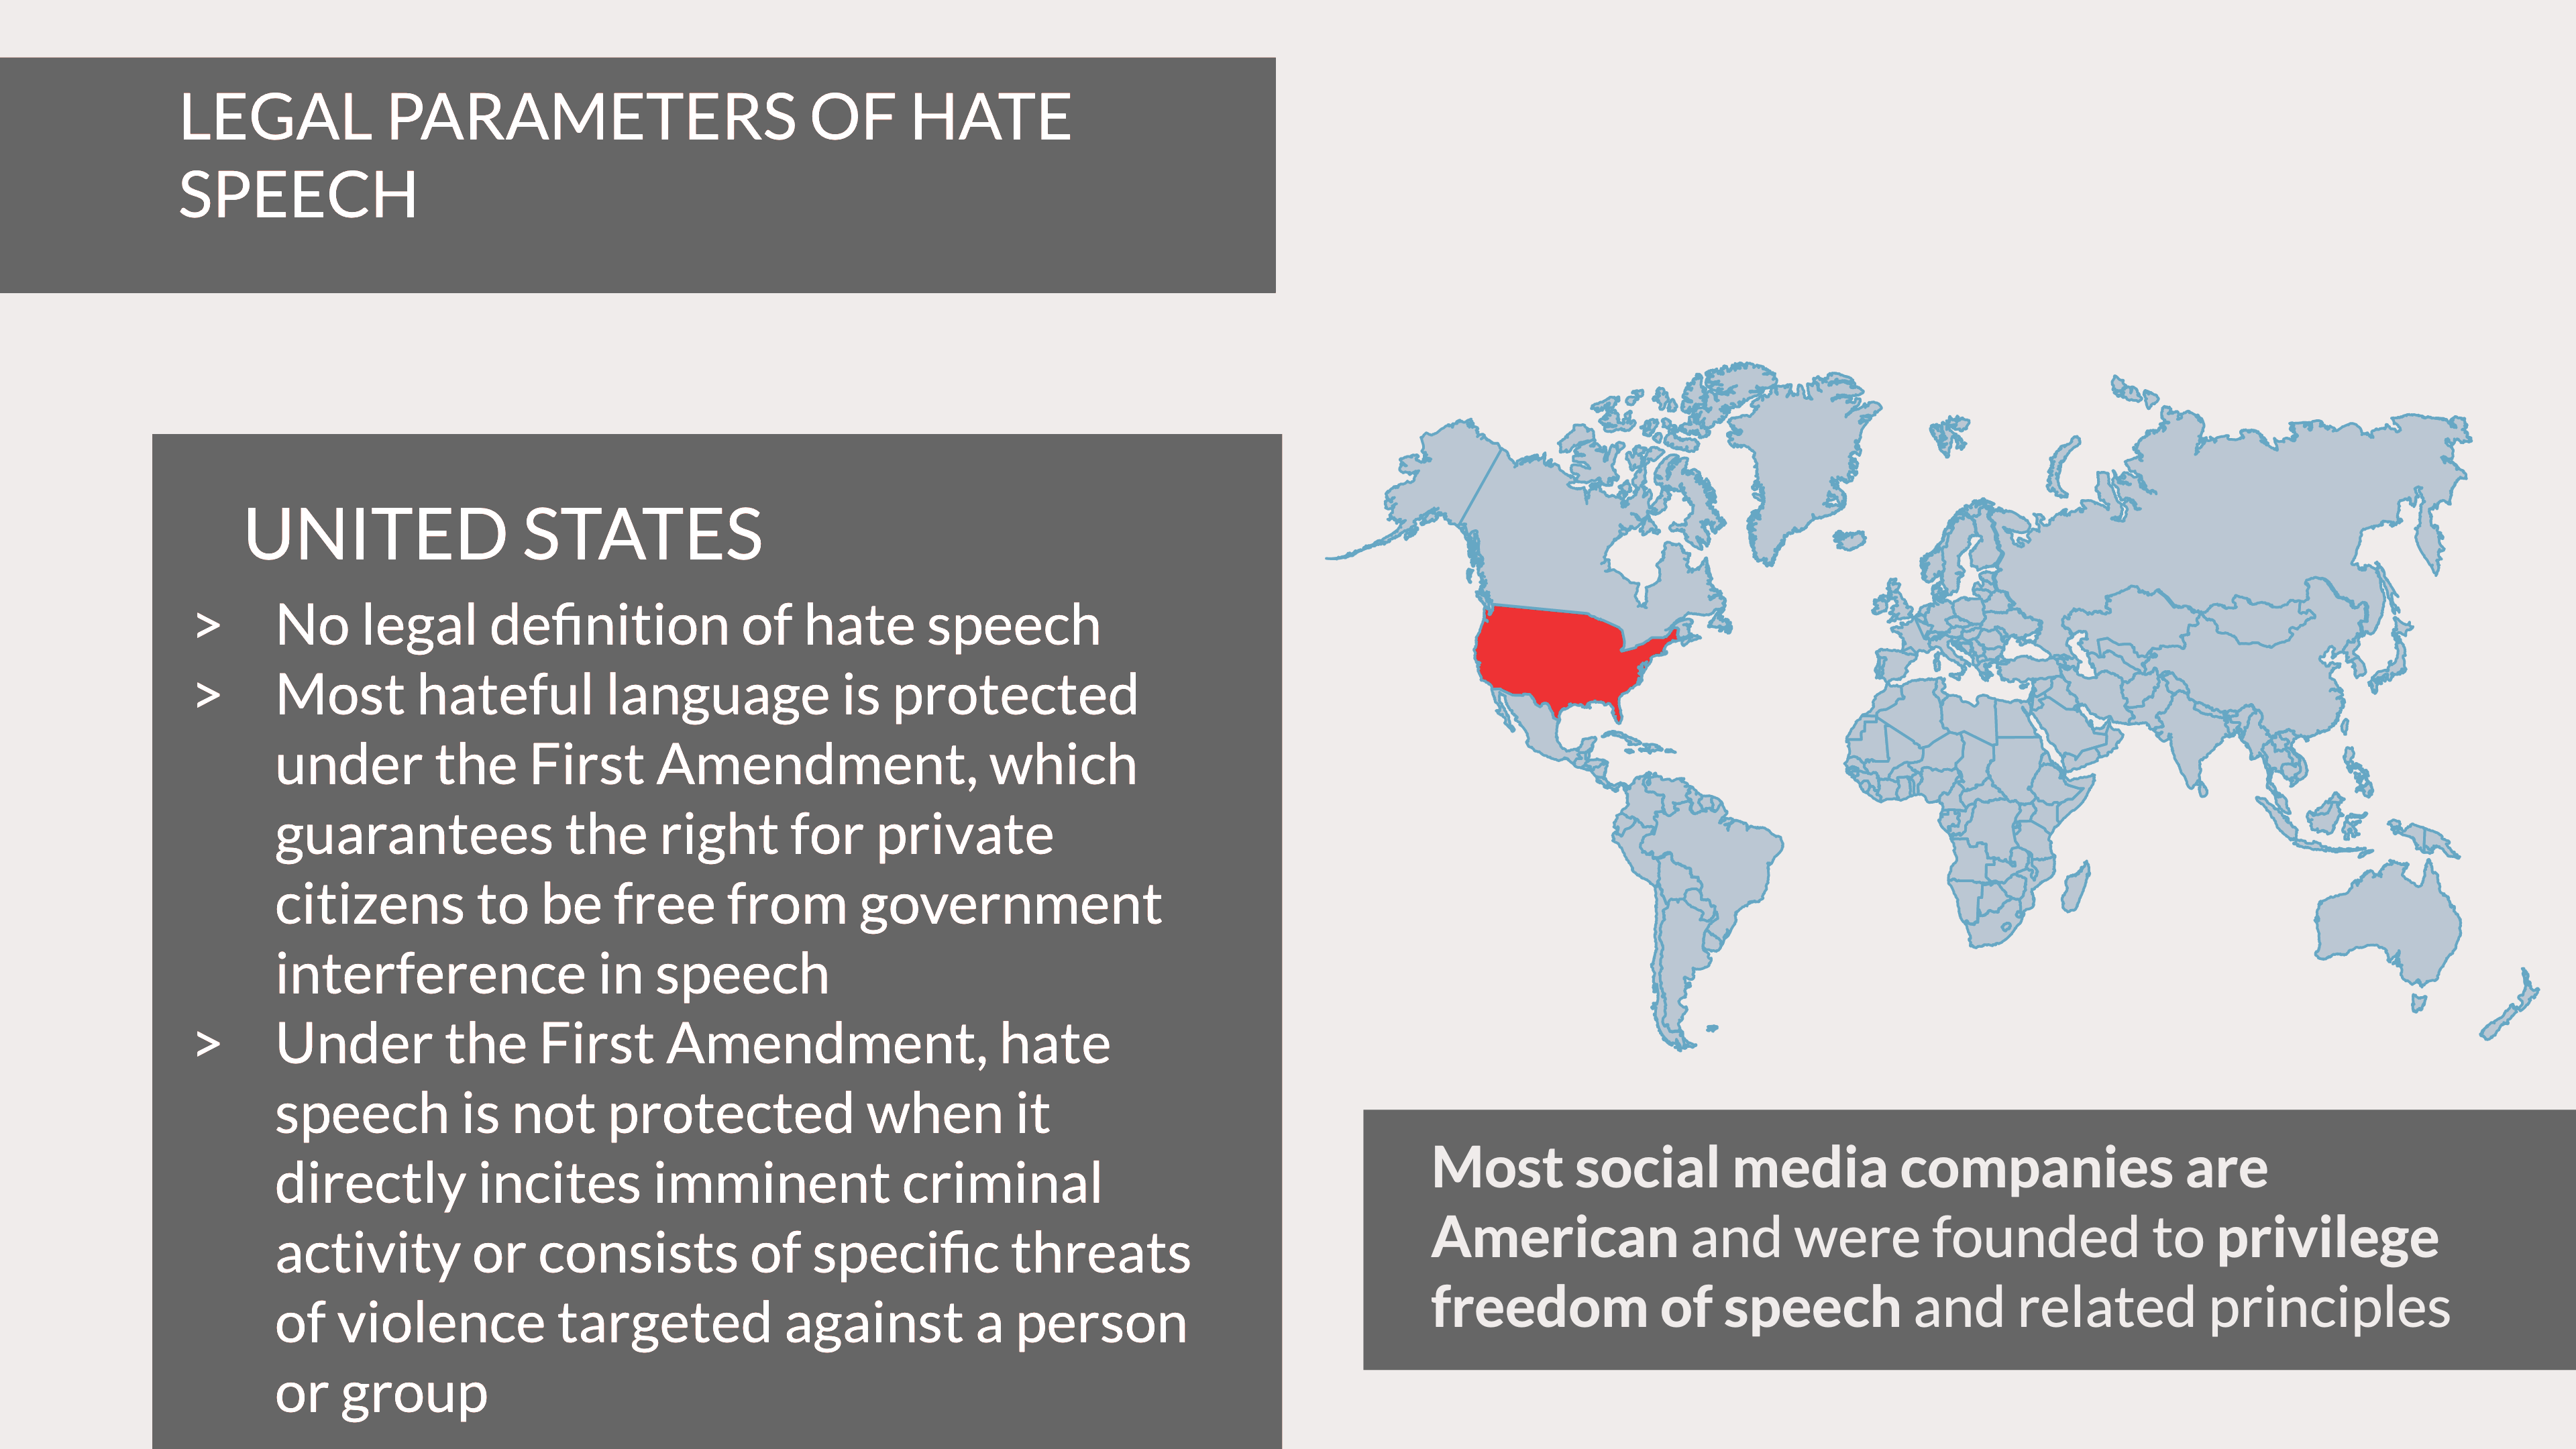
\includegraphics[width=\paperwidth]{legal-params-1}}
\end{frame}

\begin{frame}{}
    \thispagestyle{empty}
    \AddToShipoutPictureBG*{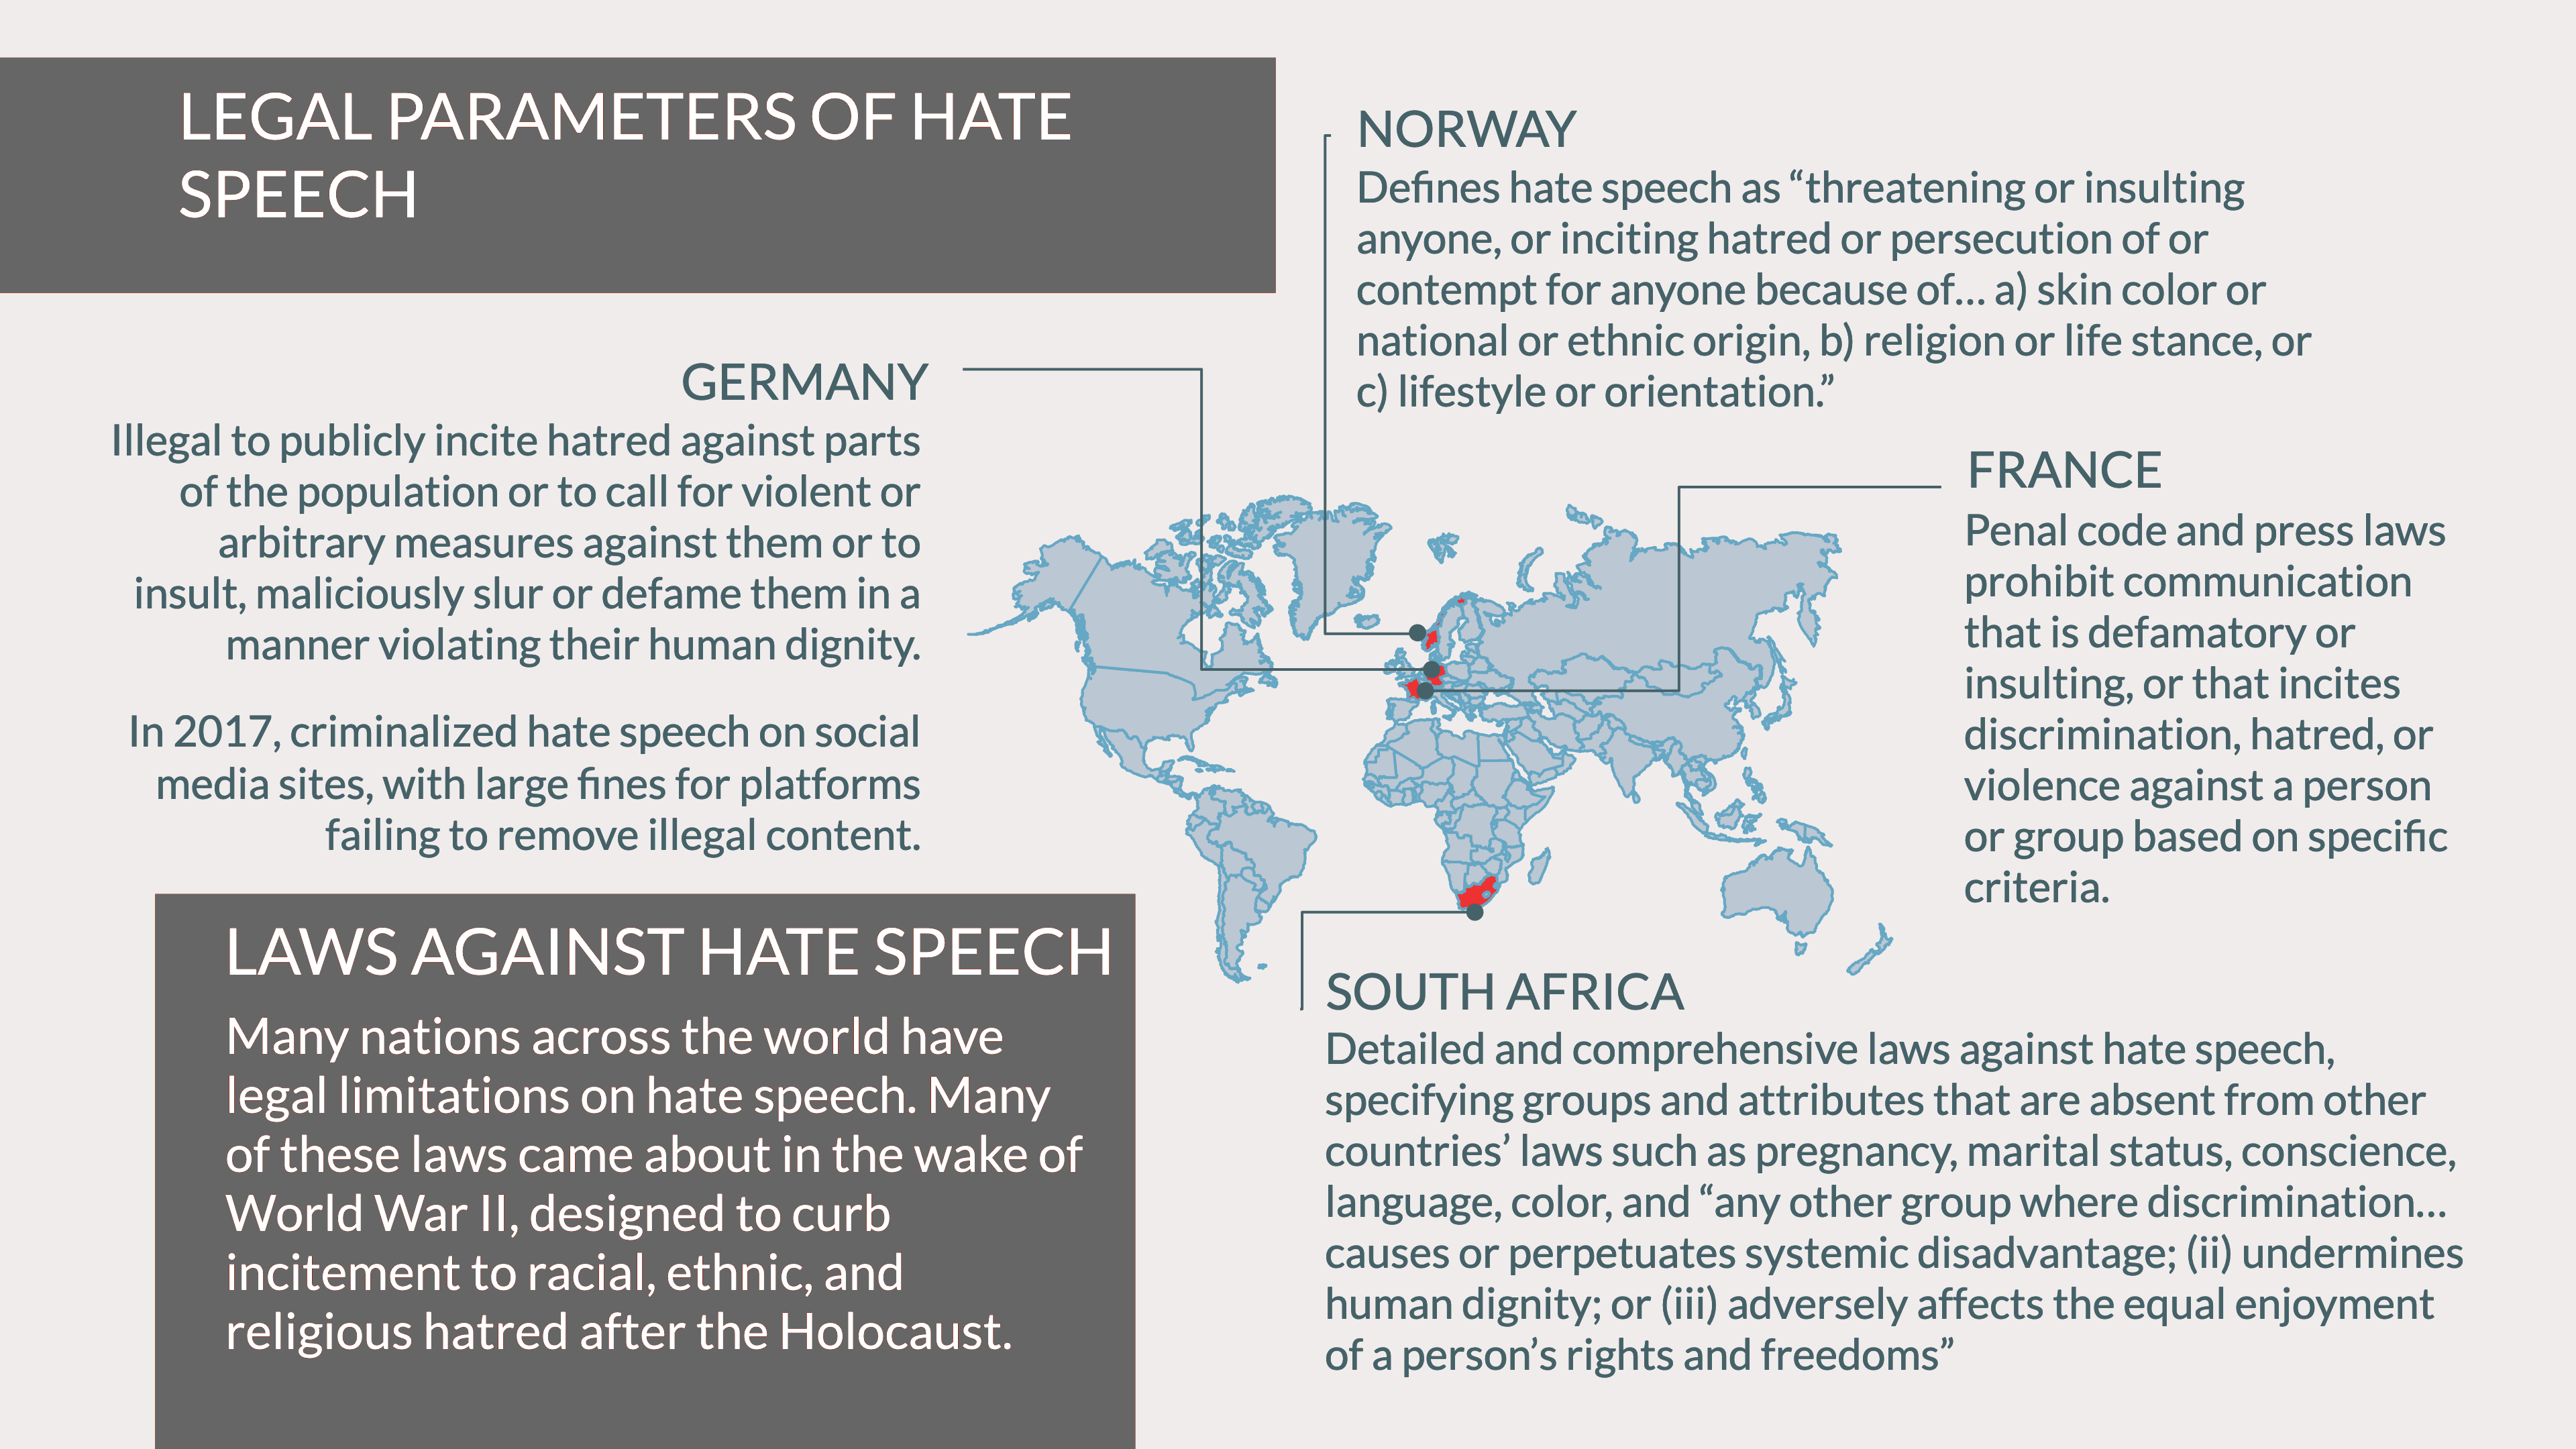
\includegraphics[width=\paperwidth]{legal-params-2}}
\end{frame}

\begin{frame}{}
    \thispagestyle{empty}
    \AddToShipoutPictureBG*{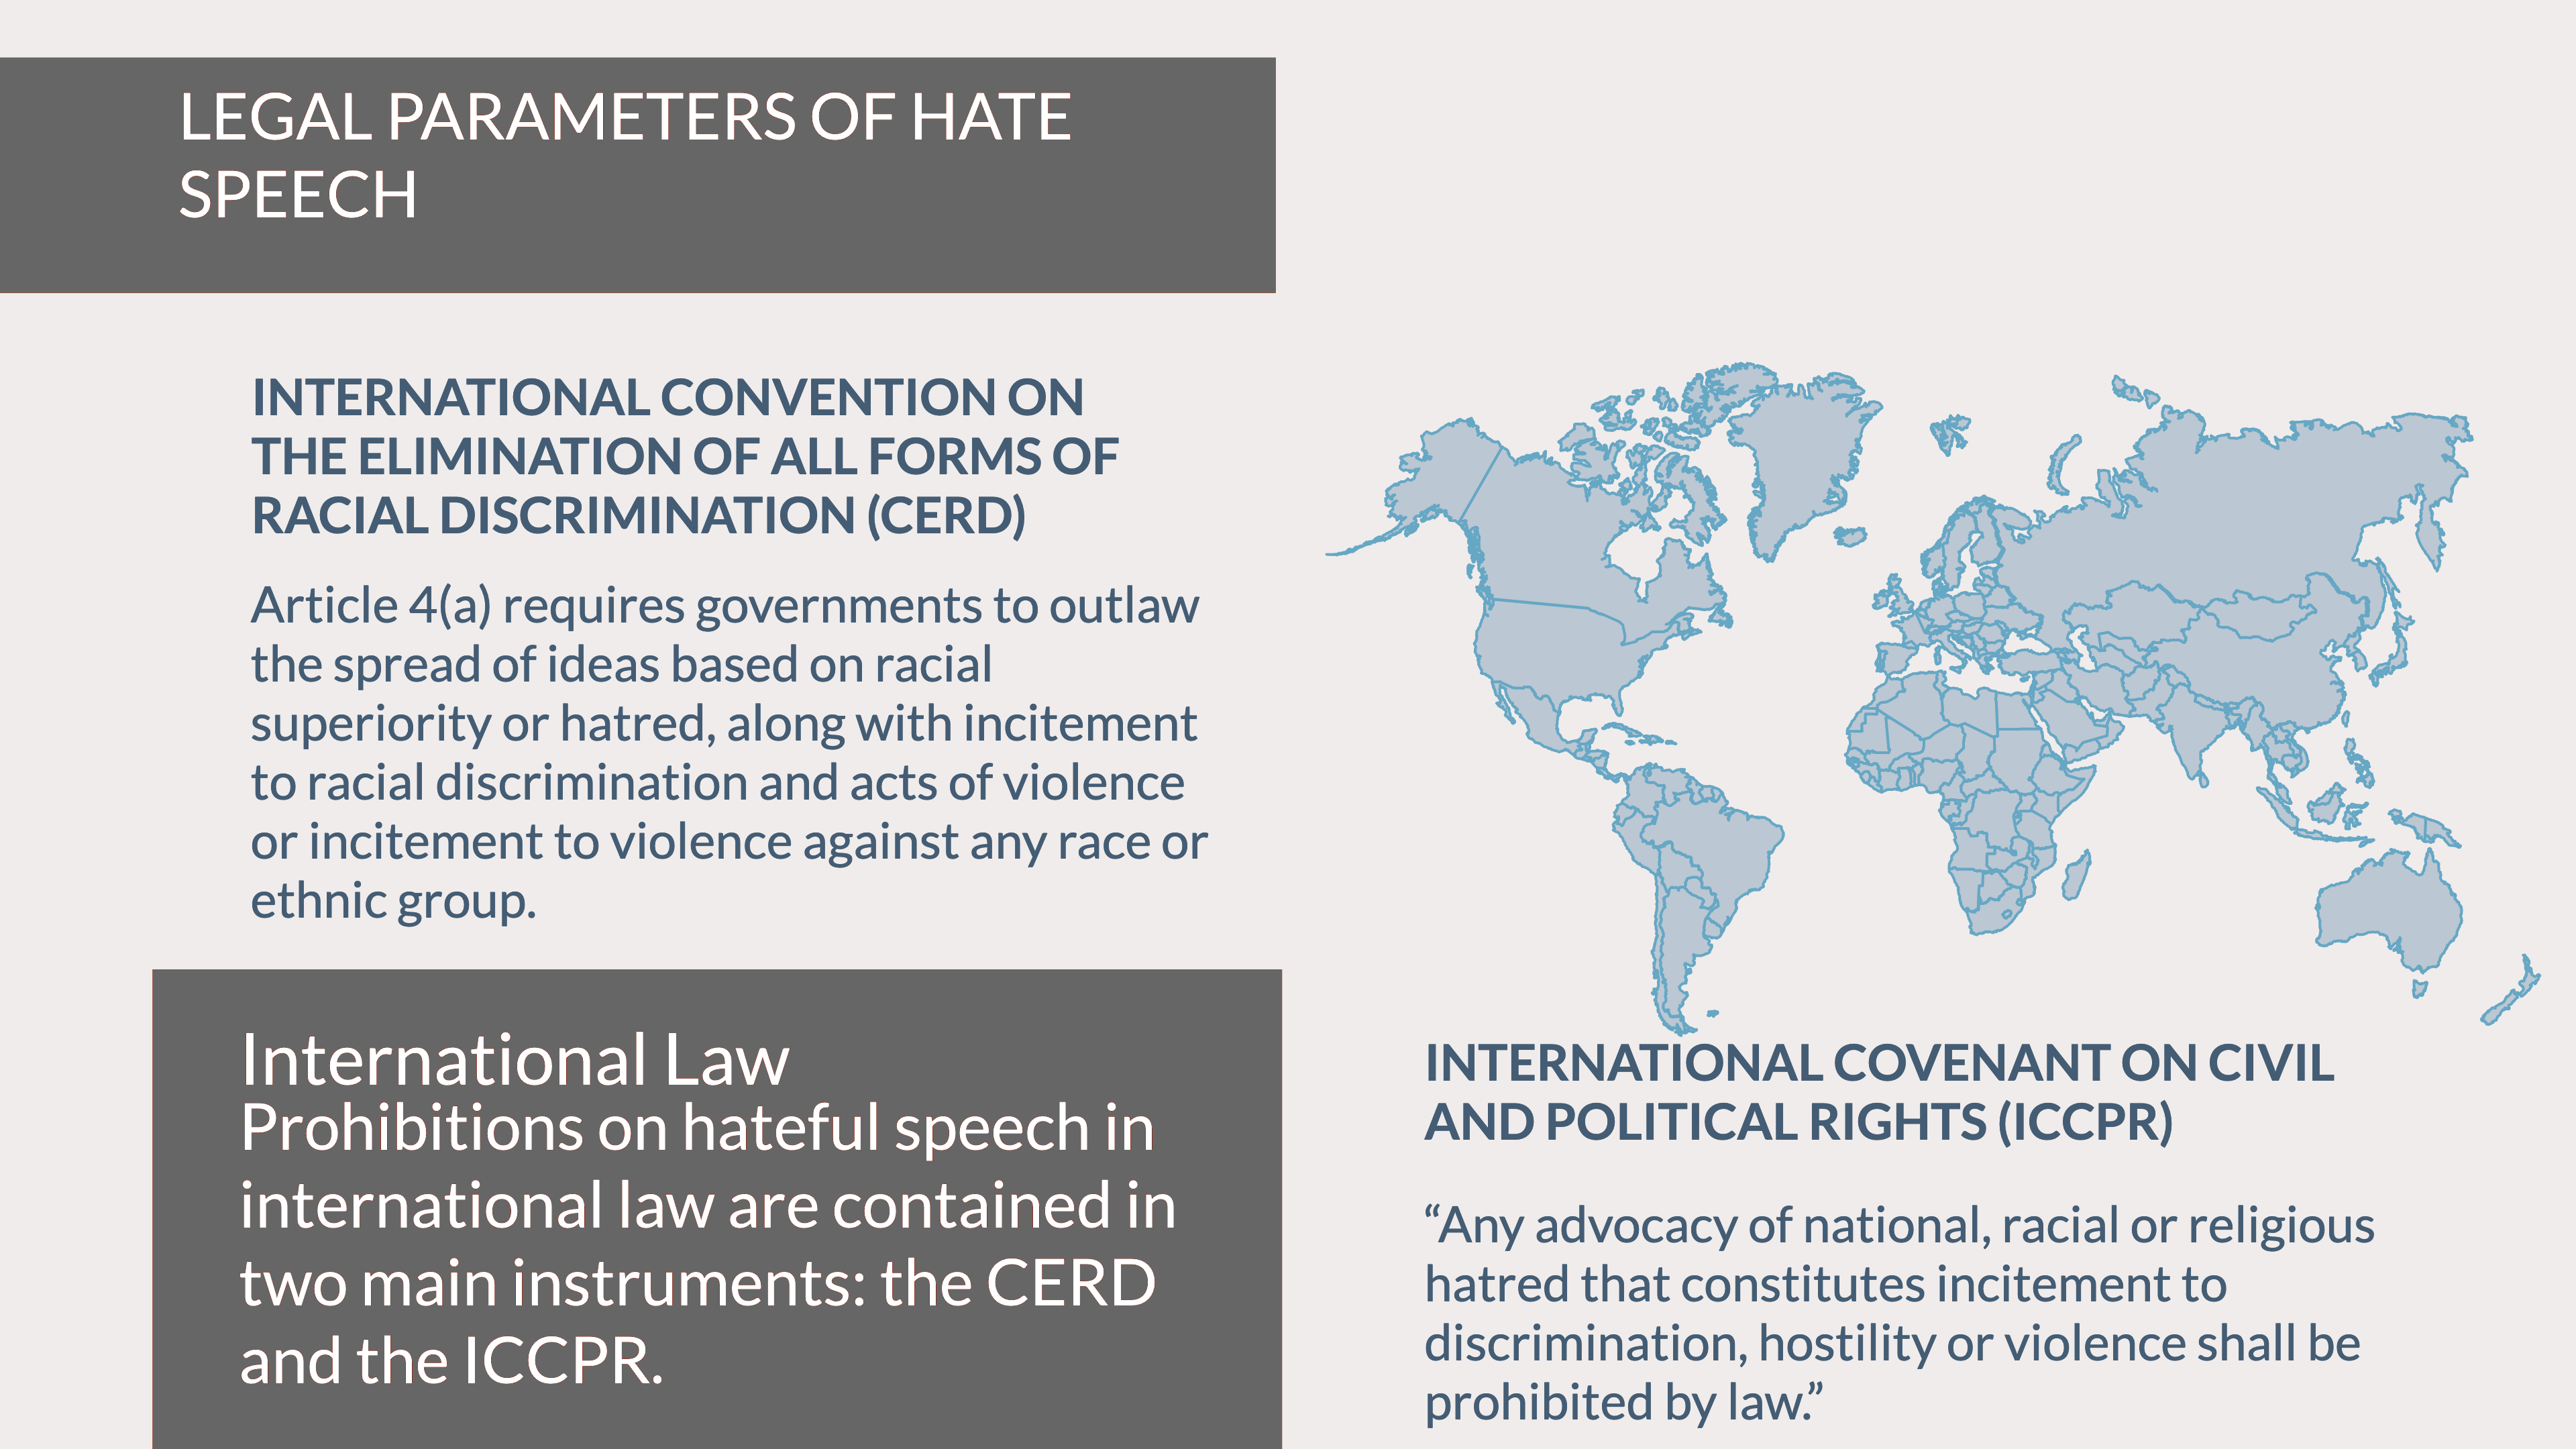
\includegraphics[width=\paperwidth]{legal-params-3}}
\end{frame}

\begin{frame}{}
    \thispagestyle{empty}
    \AddToShipoutPictureBG*{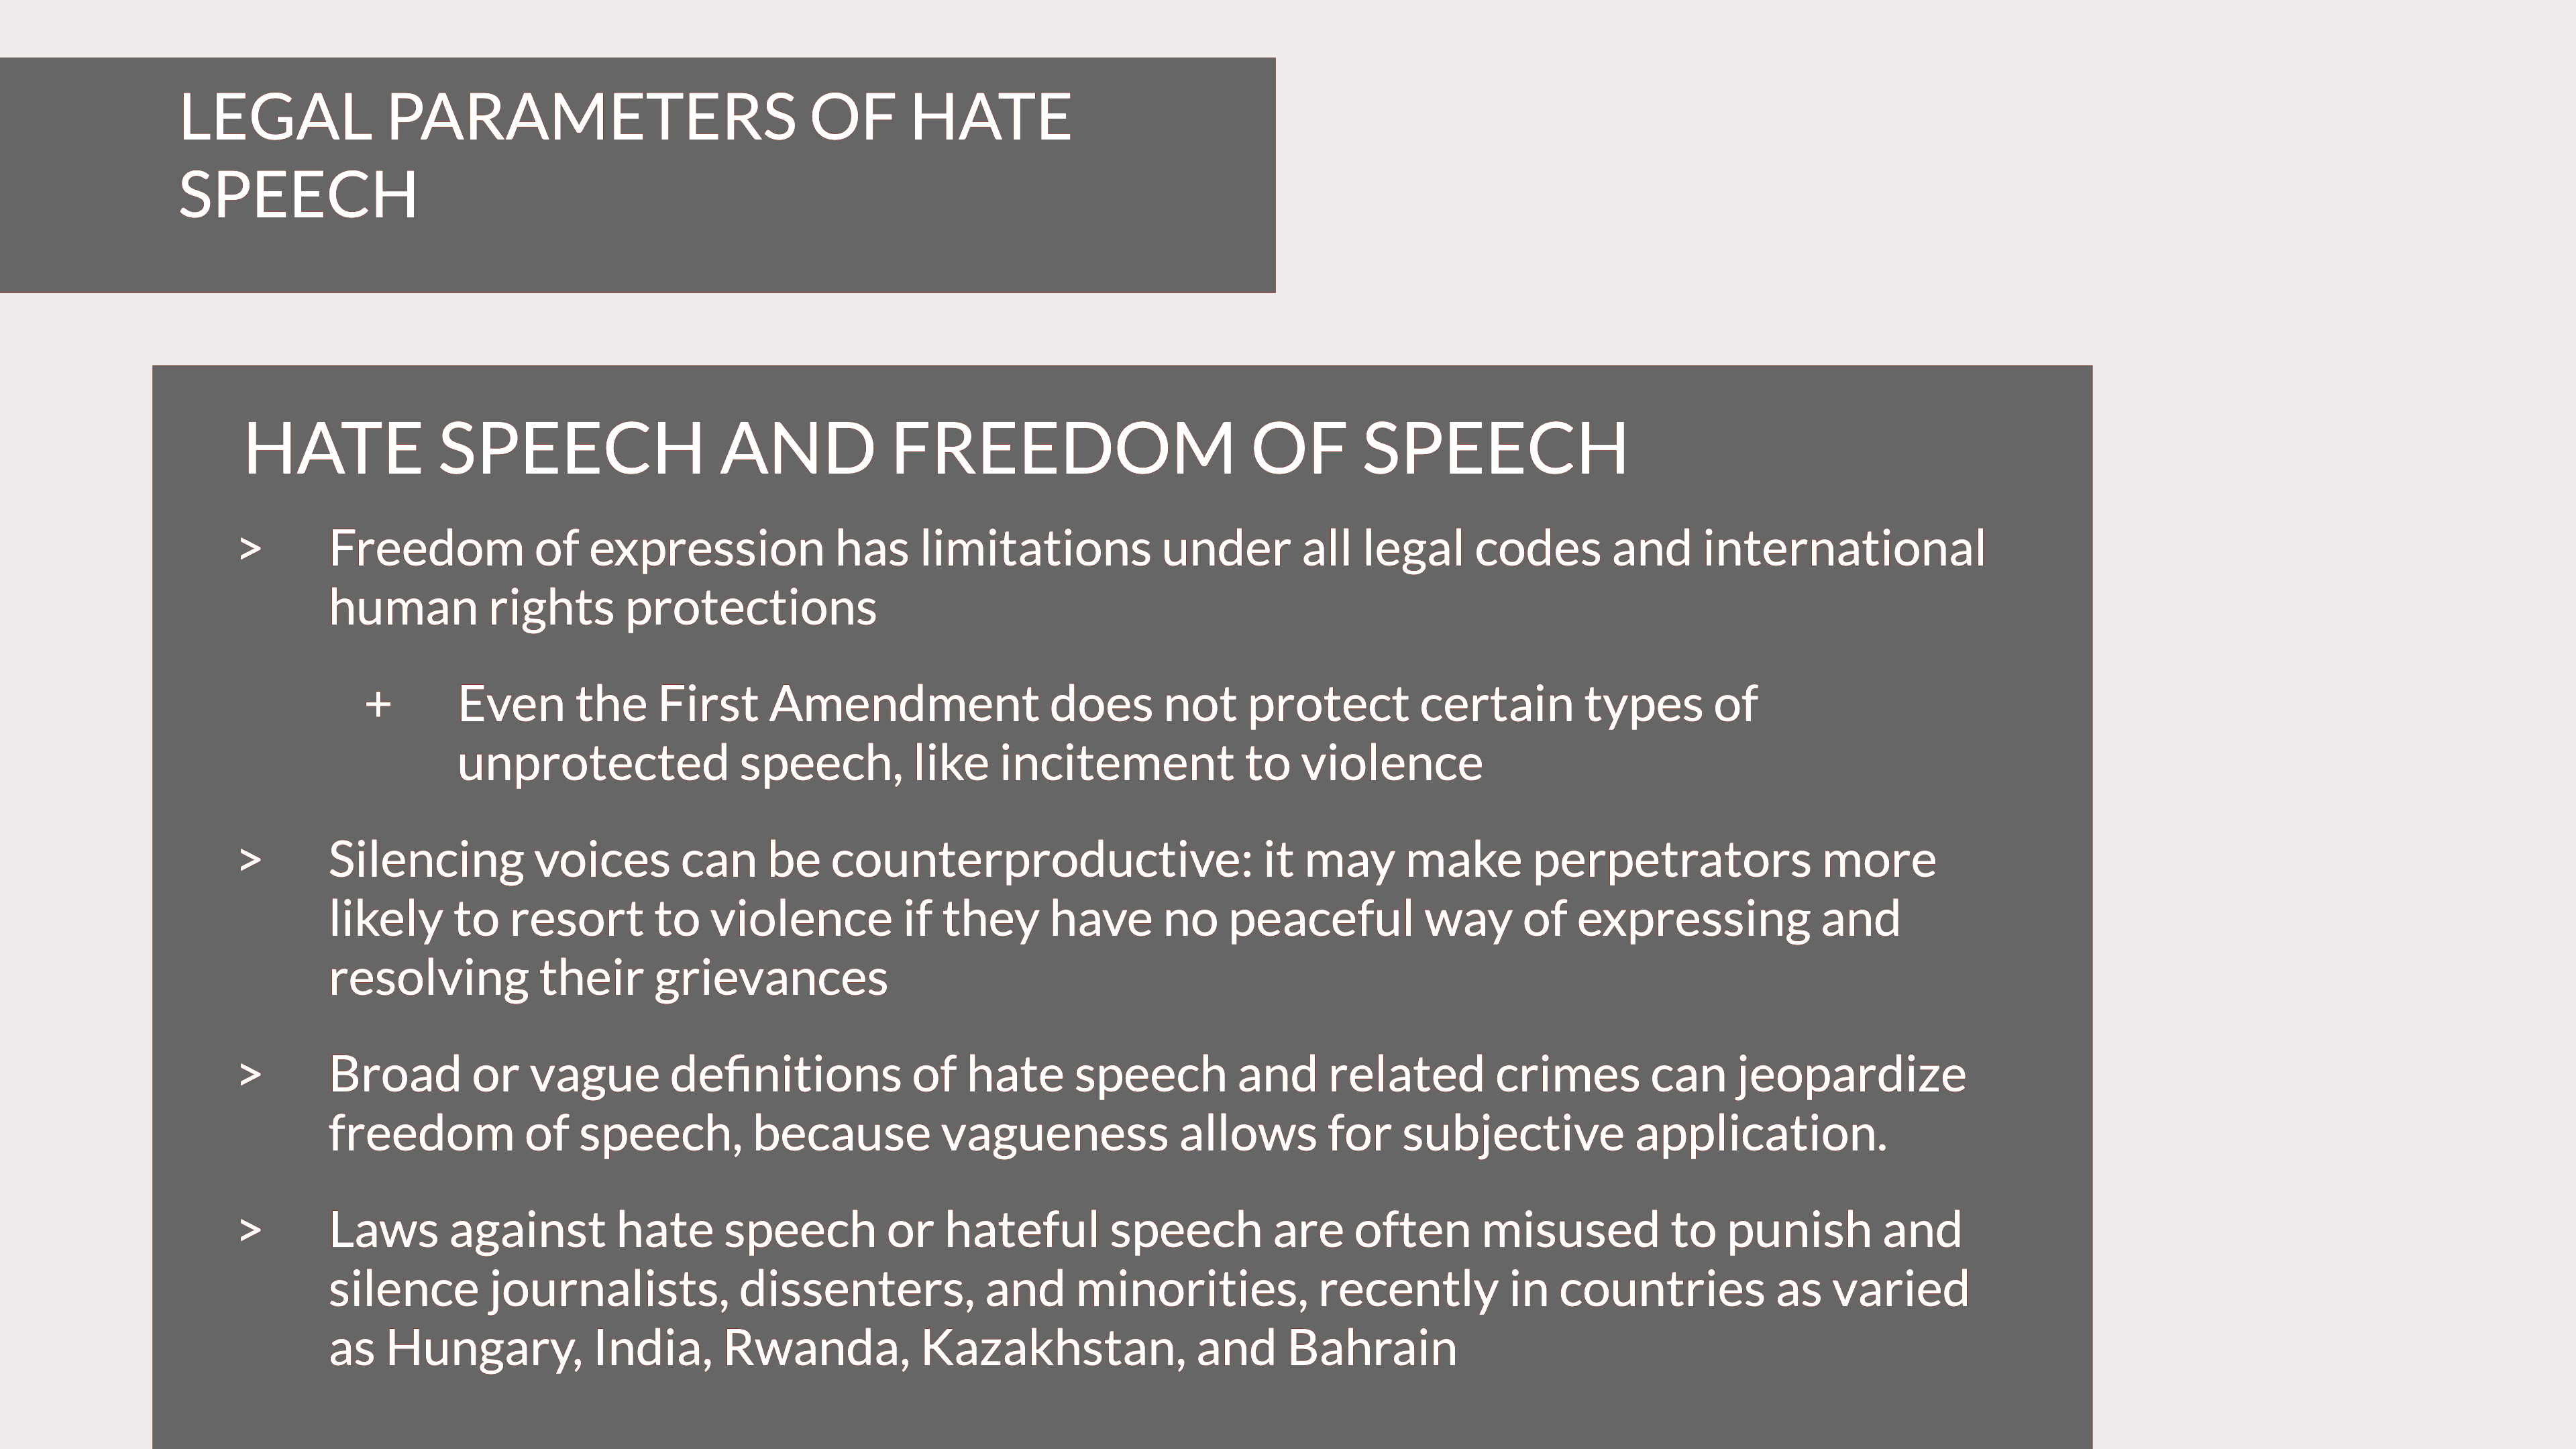
\includegraphics[width=\paperwidth]{legal-params-4}}
\end{frame}

\begin{frame}{Definitions Under International Law}
    \centering
    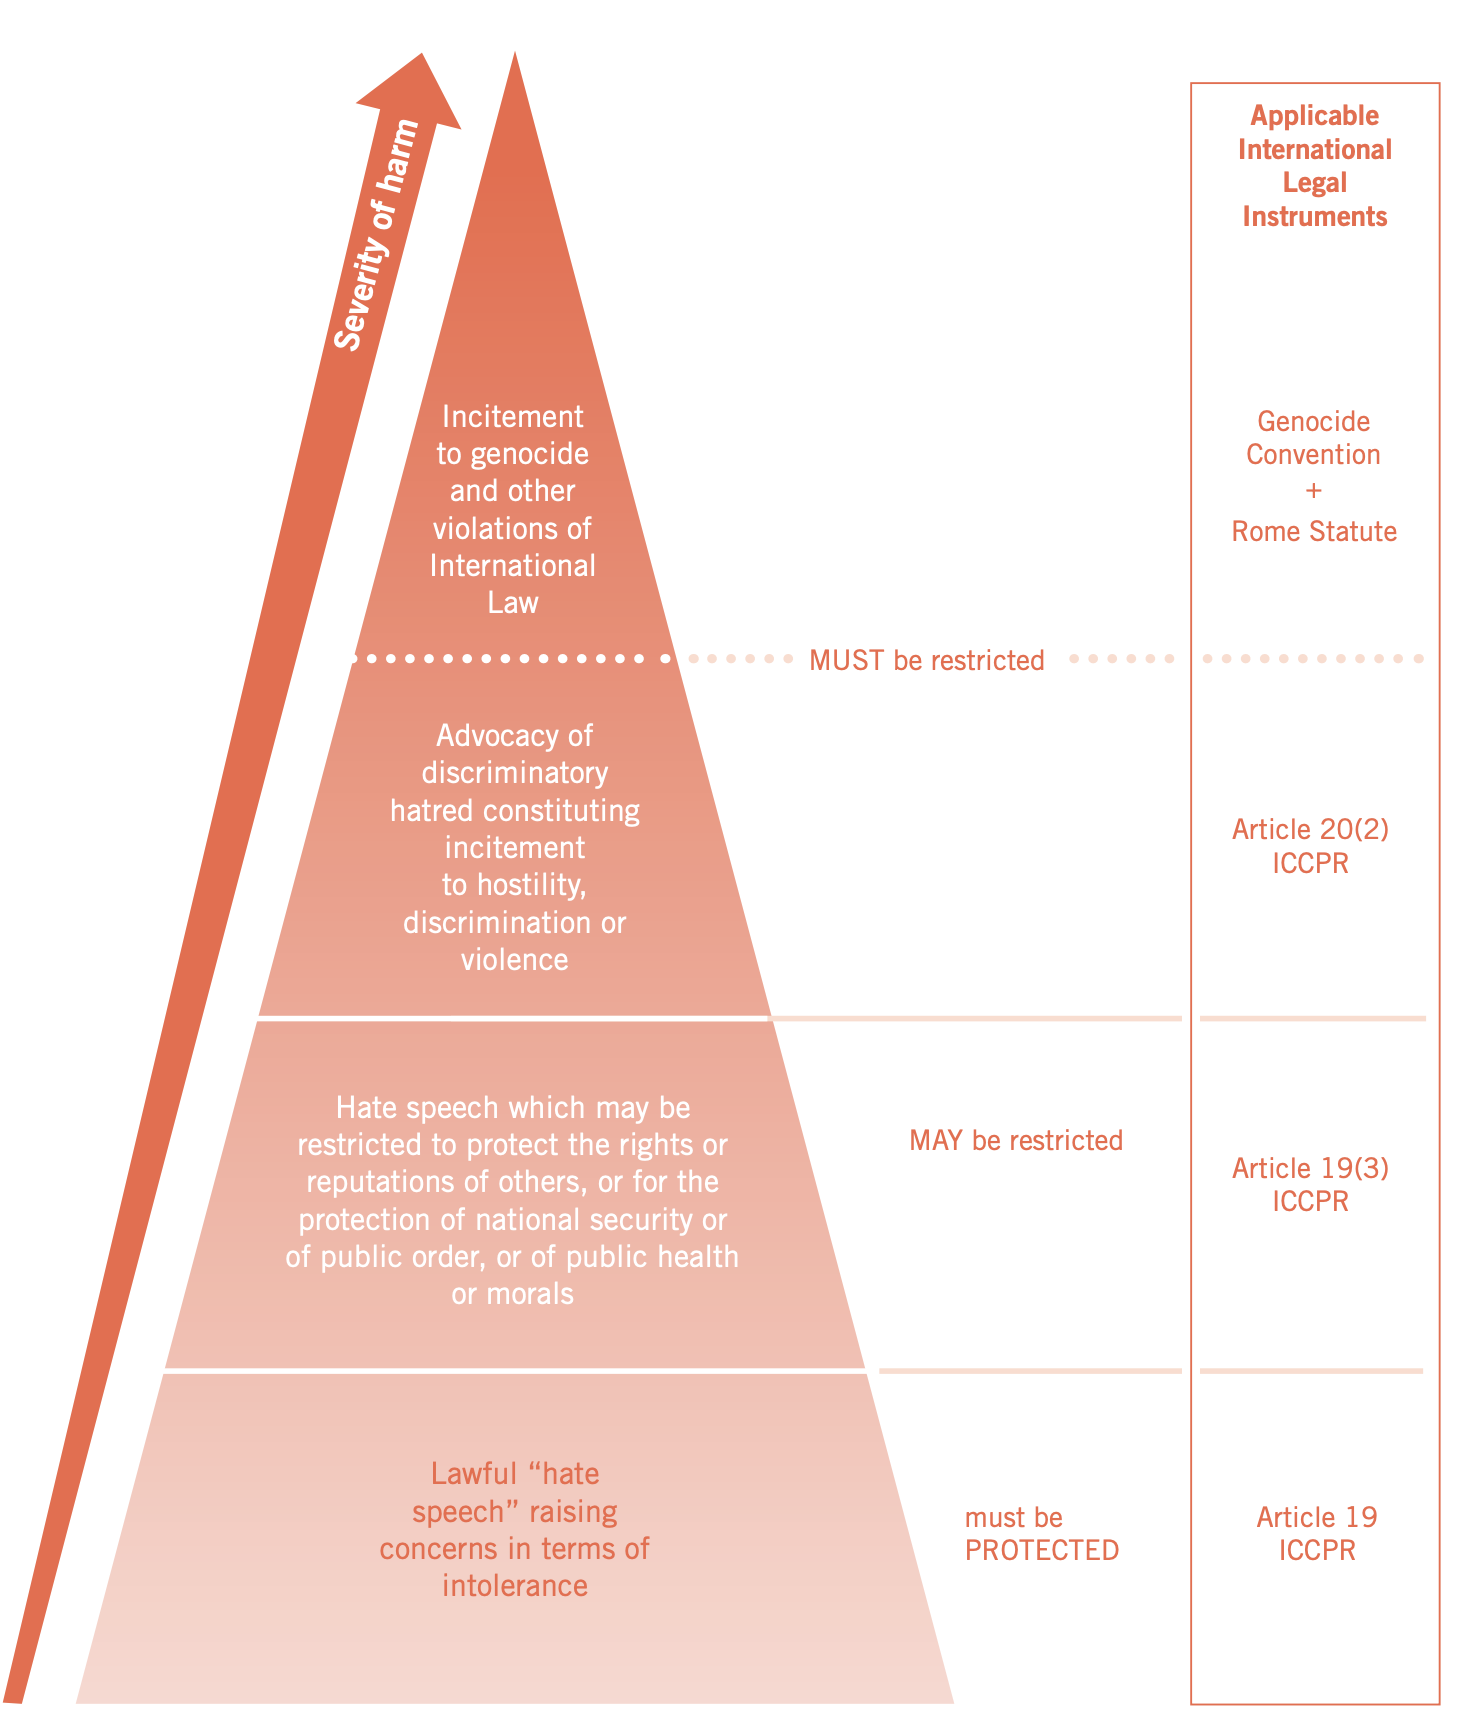
\includegraphics[height=0.8\textheight]{hate-speech-pyramid}
    \tiny
    \underline{\href{https://www.article19.org/data/files/medialibrary/38231/'Hate-Speech'-Explained---A-Toolkit-\%282015-Edition\%29.pdf}{Source: article19.org}}
    %TODO best way to source so it isn't too long
\end{frame}

\begin{frame}{Organized Hate Speech Is Often Multi-platform}
    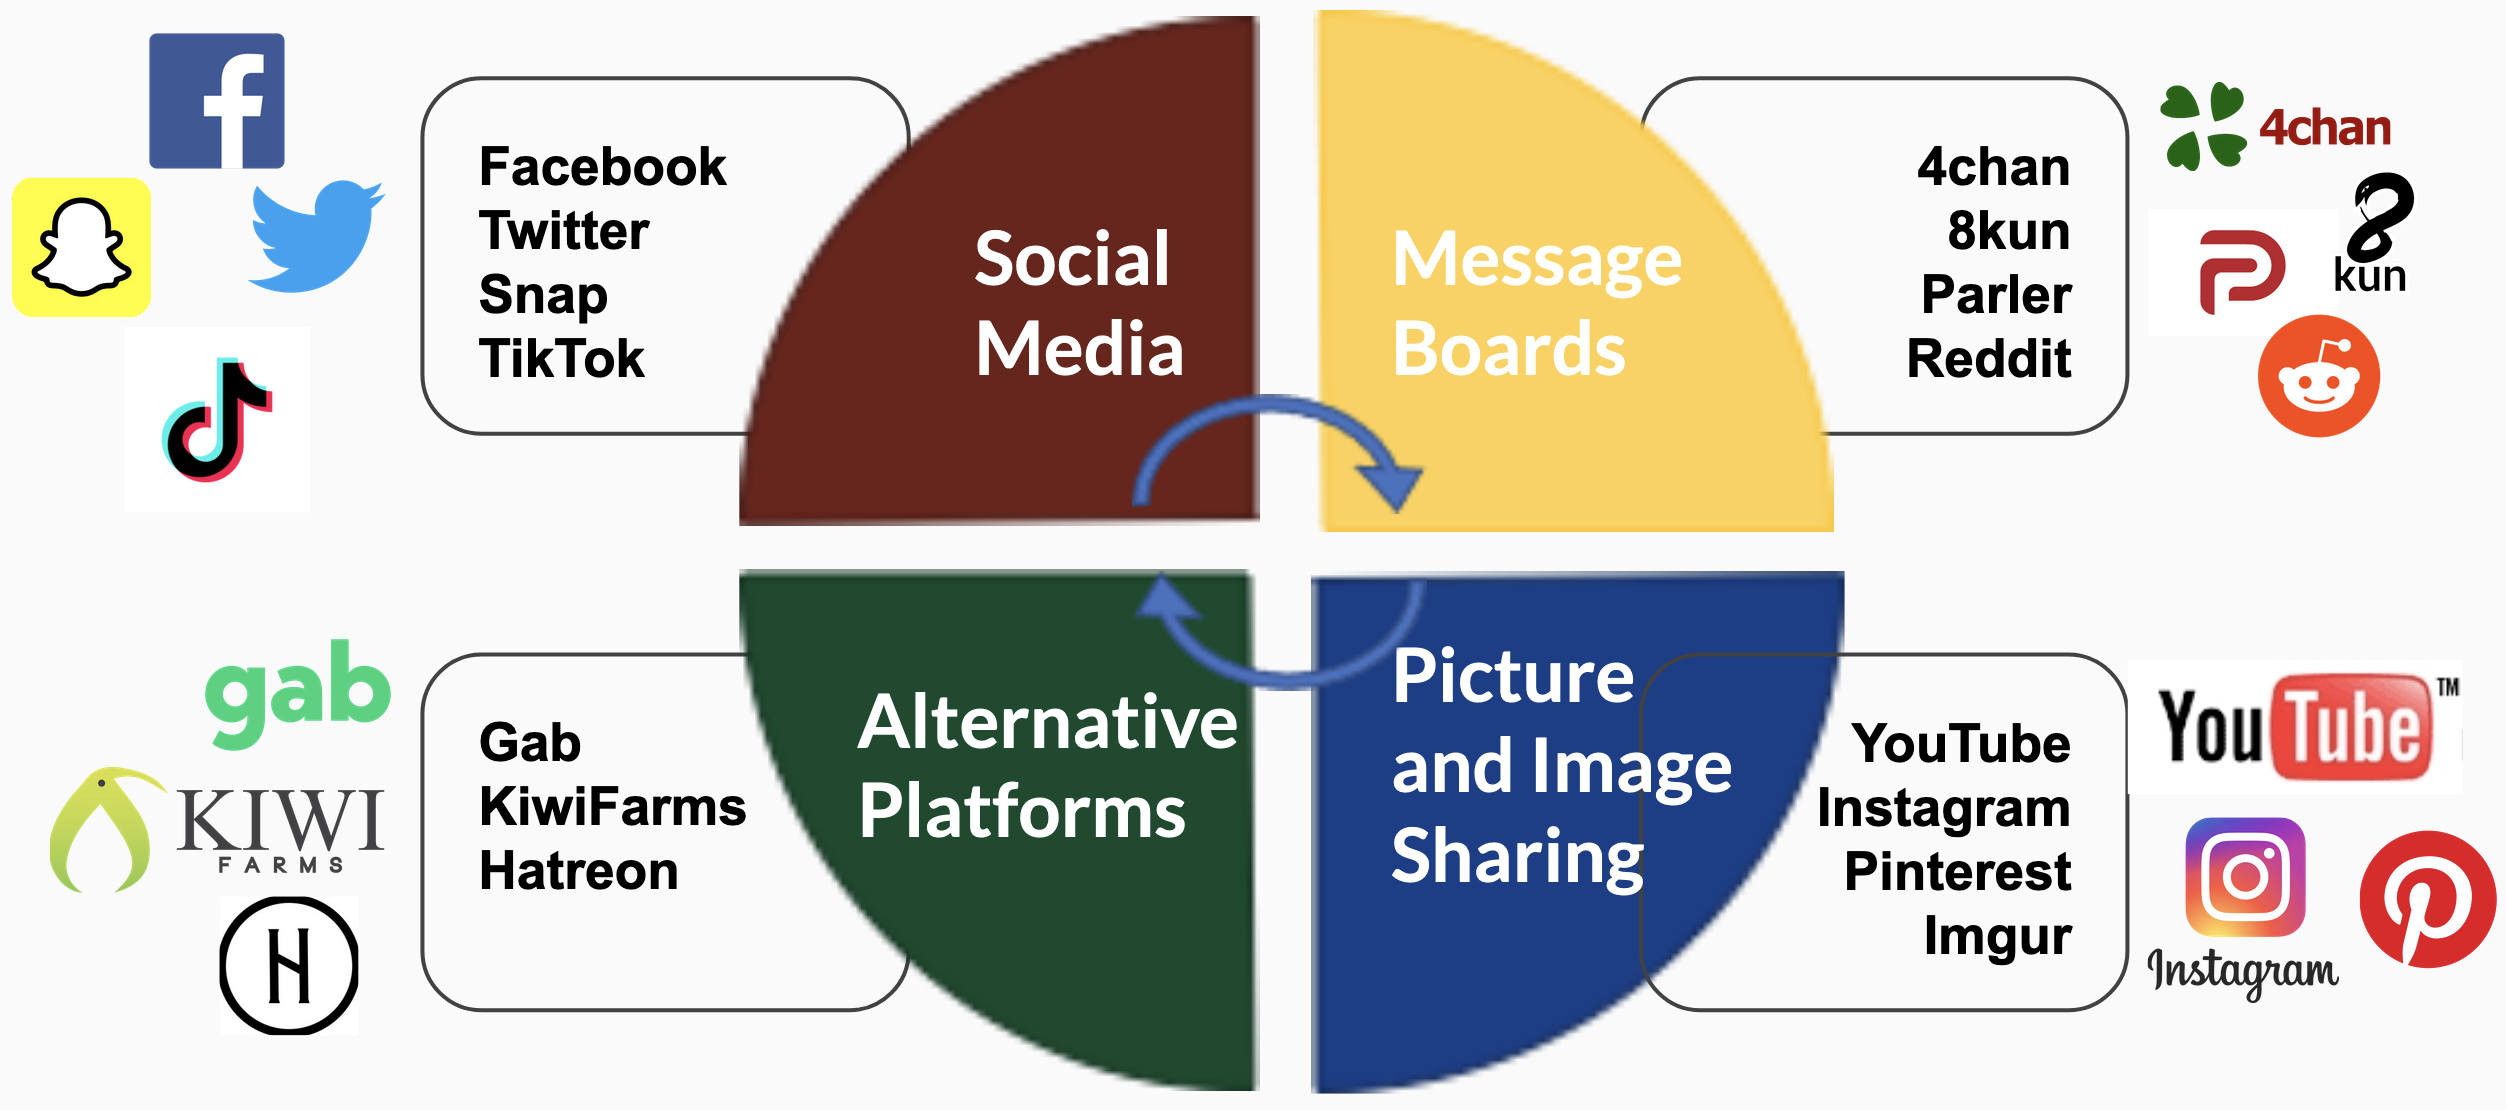
\includegraphics[width=\textwidth]{multiplatform-hate-speech}
\end{frame}

\section{Hate Speech and Incitement to Violence}

\begin{frame}{Hate Speech Is a Key Component to Ethnic Violence and Genocide}
    The Eight Stages of Genocide:
    \begin{itemize}
        \item Classification
        \item Symbolization
        \item Dehumanization
        \item Organization
        \item Polarization
        \item Preparation
        \item Extermination
        \item Denial
    \end{itemize}
    \small
    From “\underline{\href{https://www.keene.edu/academics/ah/cchgs/resources/educational-handouts/the-eight-stages-of-genocide/download/}{The Eight Stages of Genocide}}”, G. Stanton, Genocide Watch
\end{frame}

\begin{frame}{}
    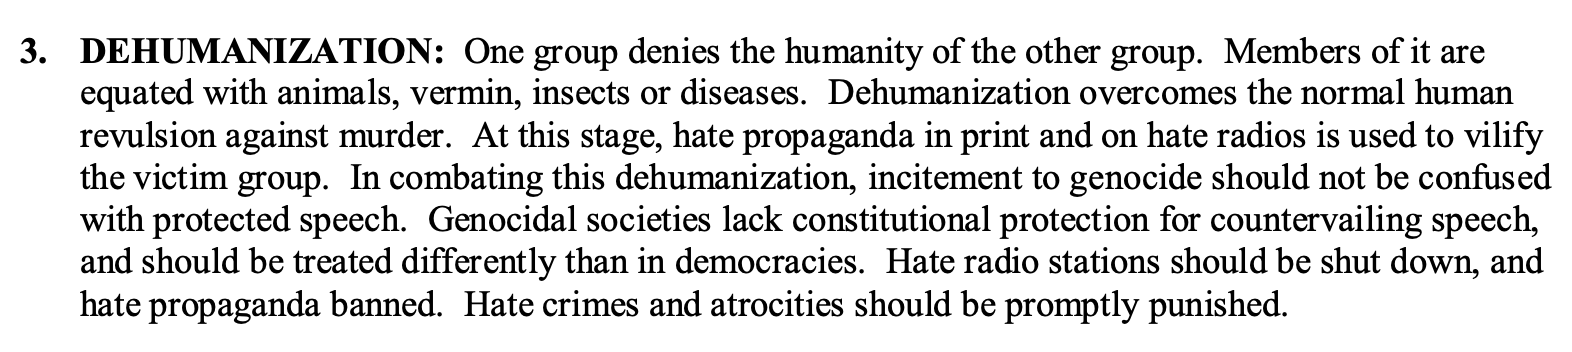
\includegraphics[width=\textwidth]{dehumanization}
    \begin{columns}
        \column{0.5\textwidth}
            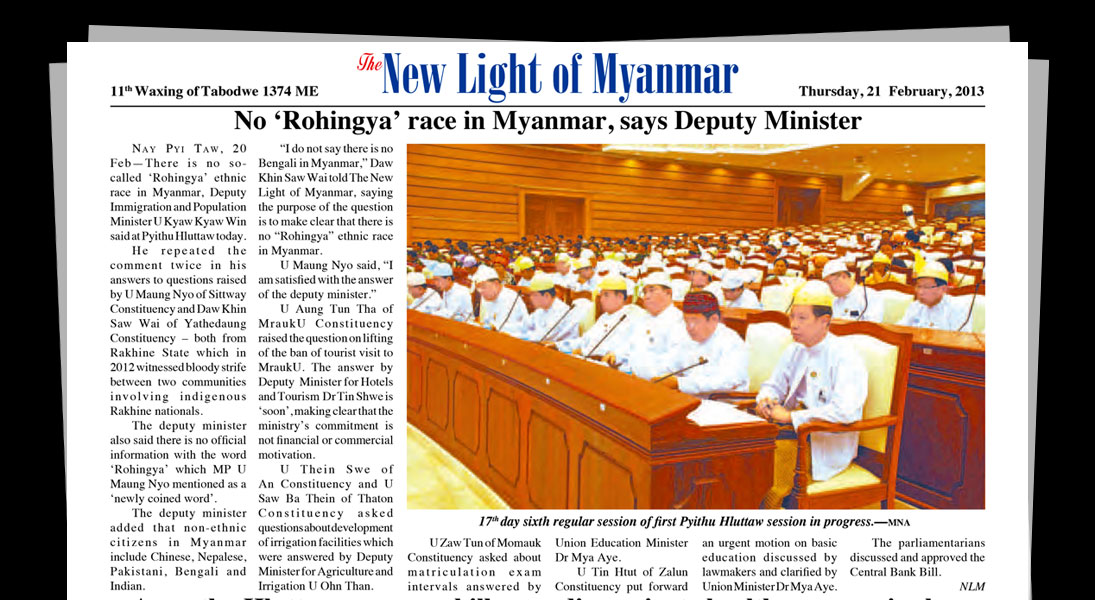
\includegraphics[width=\textwidth]{rohingya-myanmar}
        \column{0.5\textwidth}
            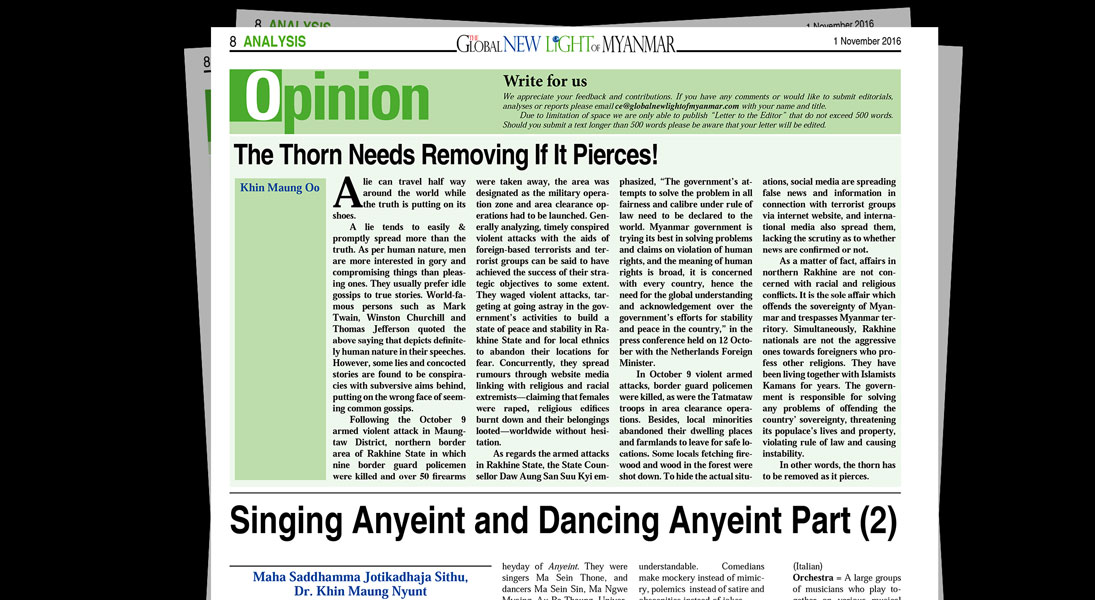
\includegraphics[width=\textwidth]{rohingya-as-a-thorn}
    \end{columns}
\end{frame}

\begin{frame}{Hate speech can easily become incitement to violence}
    \begin{columns}[T]
        \column{0.5\textwidth}
            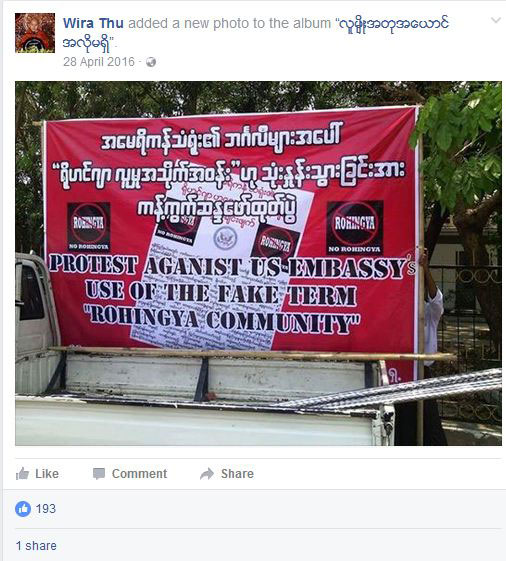
\includegraphics[width=\textwidth]{myanmar-incitement-1}
        \column{0.5\textwidth}
            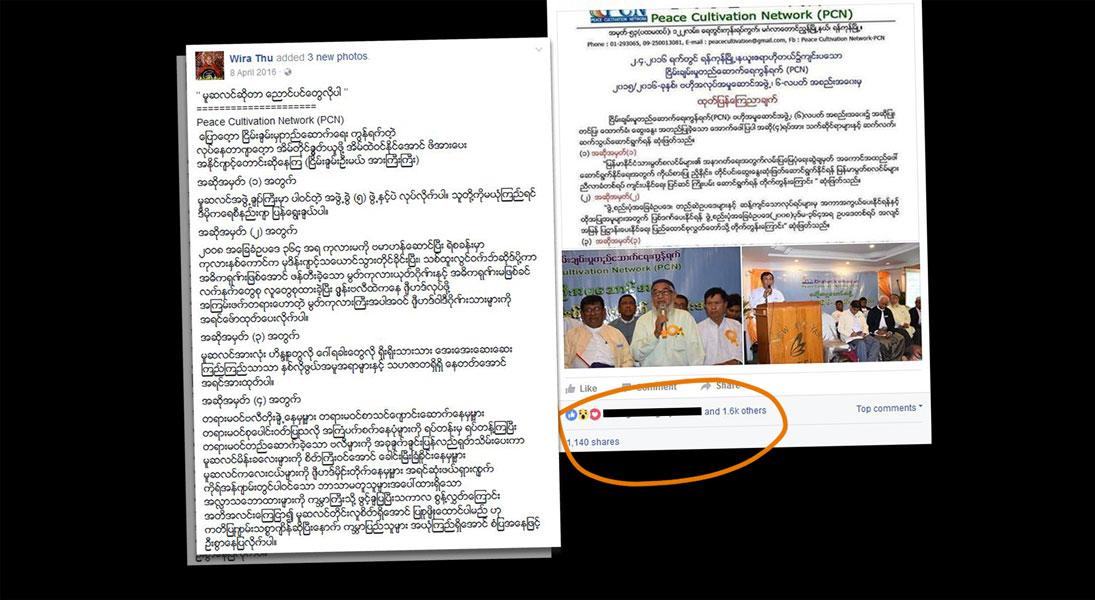
\includegraphics[width=\textwidth]{myanmar-incitement-2}
            \footnotesize
            “Muslims are like Banyan Trees - If a banyan tree grows on the idol statues, the idol statues get destroyed. If you don’t want to sugar from the Muslim’s destructions, send them away. I mean send them away from human society.”
    \end{columns}
    \tiny
    \url{https://exhibitions.ushmm.org/burmas-path-to-genocide/chapter-3/hate-speech-that-targets-rohingyas-humanity}
\end{frame}

\begin{frame}{} 
    \href{https://youtu.be/wOTYwFr3cwU}{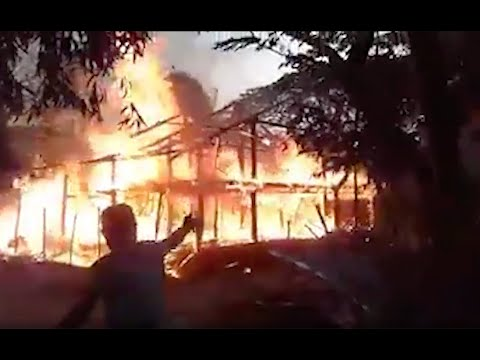
\includegraphics[width=\textwidth]{myanmar-homes-burning}}
\end{frame}

\begin{frame}{Roots of Facebook’s Failure in Myanmar}
    \large
    \begin{enumerate}
        \item Unconstrained hyper-growth and I18N
        \item Lack of content policy knowledge
        \item Government-sponsored genocide, no legal protections and mass media control
        \item No employees on the ground due to government feedback loop
        \item No AI/ML capability
        \item Extremely limited content moderation teams in relevant languages
        \item Content moderators drawn from the ethnic “winners”
    \end{enumerate}
\end{frame}

\section{Responses and Mitigations}

\begin{frame}{Policy Responses}
    \large
    \begin{enumerate}
        \item Set clear policies with the goal of optimizing the user experience
        \item Allow for complicated contexts, including criticism and counter-speech
        \item Stay aware of shifting meanings in the cultures in which you operate
    \end{enumerate}
\end{frame}

\begin{frame}{}
    \thispagestyle{empty}
    \AddToShipoutPictureBG*{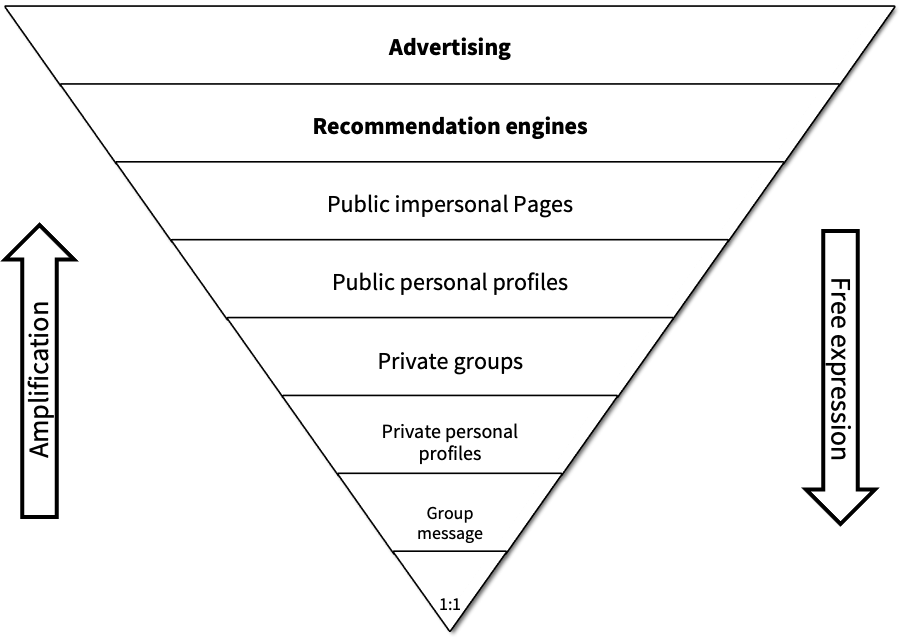
\includegraphics[width=\paperwidth]{amplification-pyramid}}
\end{frame}

\begin{frame}{}
    \thispagestyle{empty}
    \AddToShipoutPictureBG*{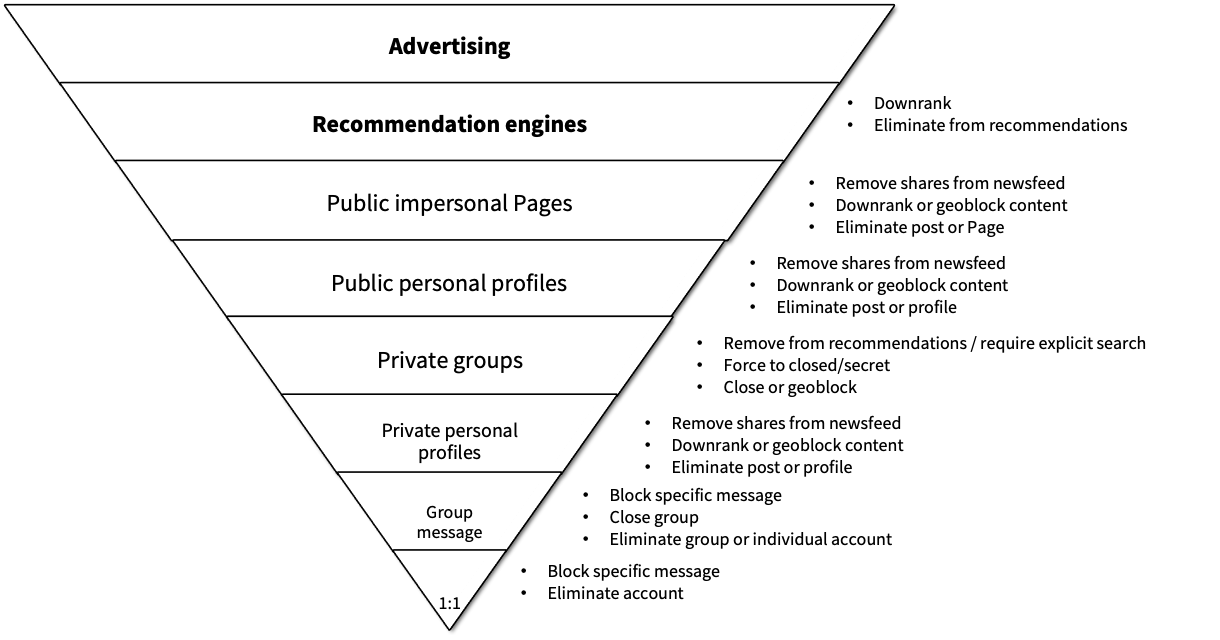
\includegraphics[width=\paperwidth]{amplification-pyramid-policies}}%TODO can't line up with top of page
\end{frame}

\begin{frame}{Context Matters}
    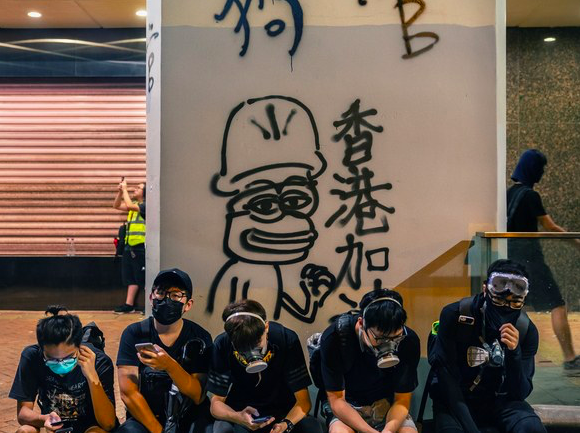
\includegraphics[width=\textwidth]{pepe-protest}
\end{frame}

\begin{frame}{Can You Find Hatespeech with a Keyword Search?}
    \begin{columns}
        \column{0.5\textwidth}
            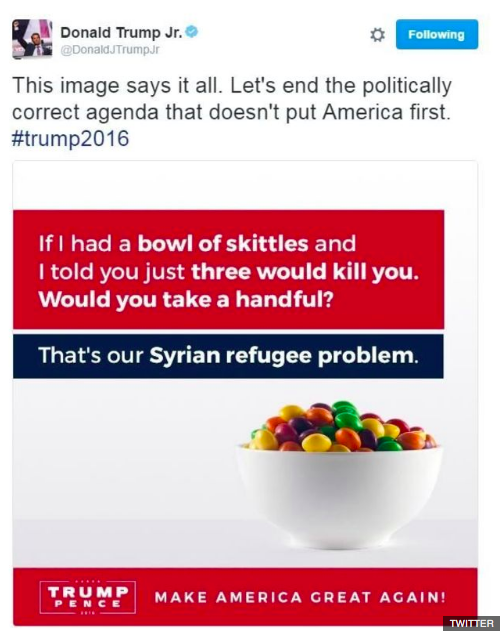
\includegraphics[width=\textwidth]{skittles}
        \column{0.5\textwidth}
             \LARGE
             \centering
             “Skittles,” and “skypes,” and “googles”...oh my.
    \end{columns}
\end{frame}

\begin{frame}{Active Co-opting of Popular Symbols}
    \begin{columns}
        \column{0.5\textwidth}
            \includegraphics[width=\textwidth]{ok-symbol-uncle-sam}
        \column{0.5\textwidth}
            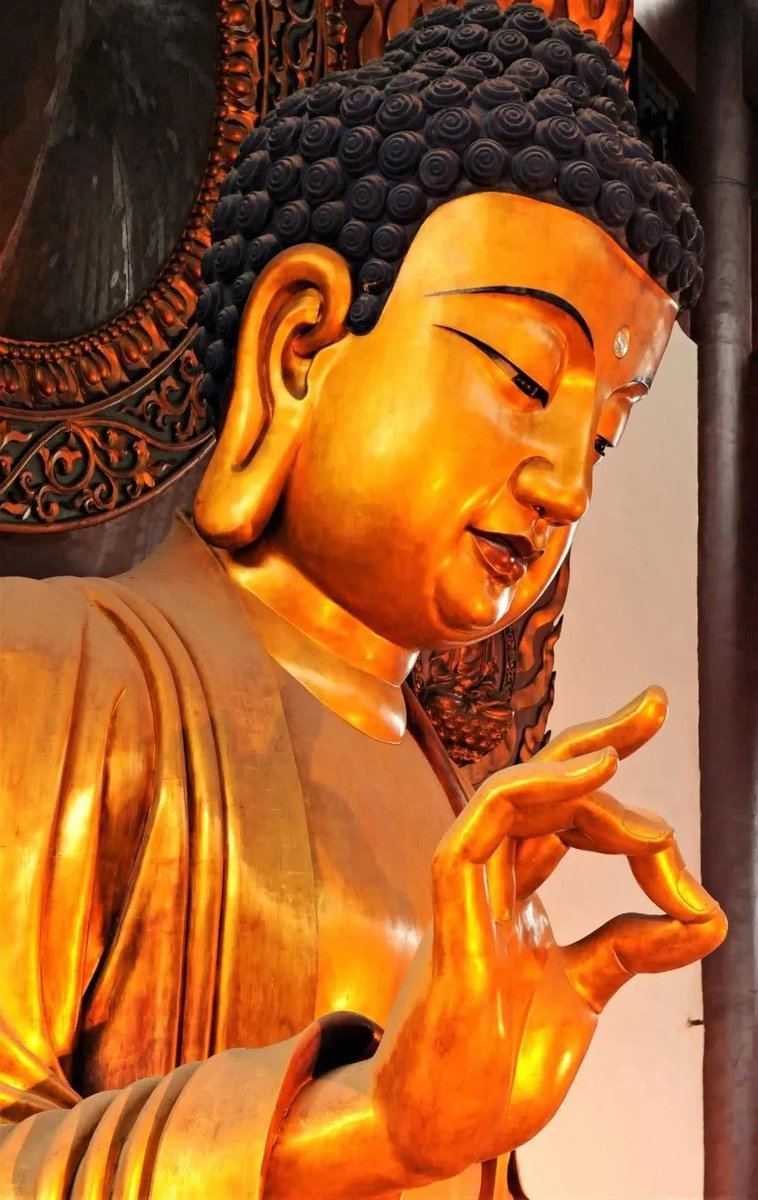
\includegraphics[width=0.9\textwidth]{ok-vitarka-mudra}
    \end{columns}
\end{frame}

\begin{frame}{Is It Real or Ironic?}
    \begin{columns}
        \column{0.6\textwidth}
            \centering
            
\includegraphics[width=\textwidth]{ok-symbol-4chan}
            
\includegraphics[width=0.5\textwidth]{ok-symbol-brenton-tarrant}
        \column{0.4\textwidth}
            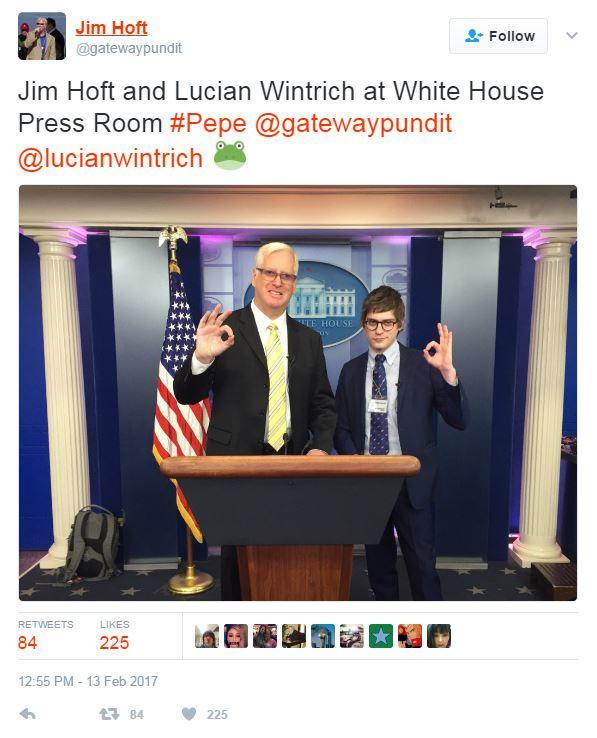
\includegraphics[width=\textwidth]{ok-symbol-hoft-wintrich}
    \end{columns}
\end{frame}

\begin{frame}{Product/Technical Responses}
    \large
    \begin{enumerate}
        \item Reporting flows
        \item Proactive monitoring
        \item Productive friction
        \item User-controls
        \item Shadow-blocking
    \end{enumerate}
\end{frame}

\begin{frame}{What Are Platforms Doing to Prevent Hate Speech?}
    \begin{columns}
        \column{0.4\textwidth}
            \footnotesize
            Platforms take a variety of actions to mitigate the spread or creation of hate speech:\\
            \begin{itemize}
                \item Blocking content outright
                \item Putting warnings or disclaimers on content
                \item Blocking users
                \item Putting users in “time out”
                \item Warning users before they post likely violating content
            \end{itemize}
            
            Which of these approaches is most effective? Challenging for T\&S teams? Challenging for product teams?
        \column{0.6\textwidth}
            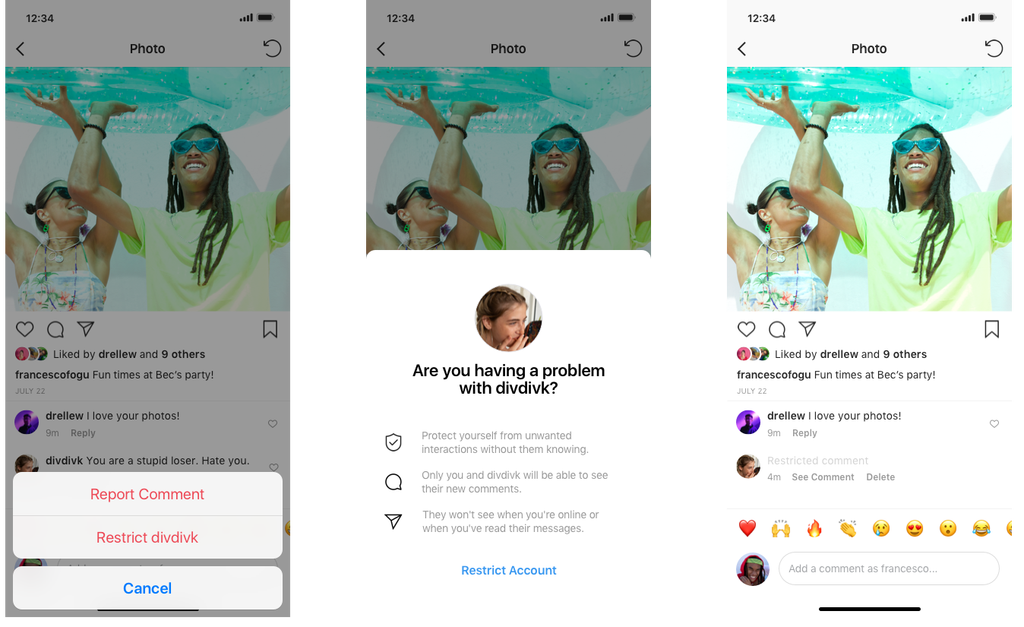
\includegraphics[width=\textwidth]{shadow-blocking}
    \end{columns}
\end{frame}

\begin{frame}{Limits of AI}
    \centering{
\includegraphics[width=0.5\textwidth]{vox-recode}
    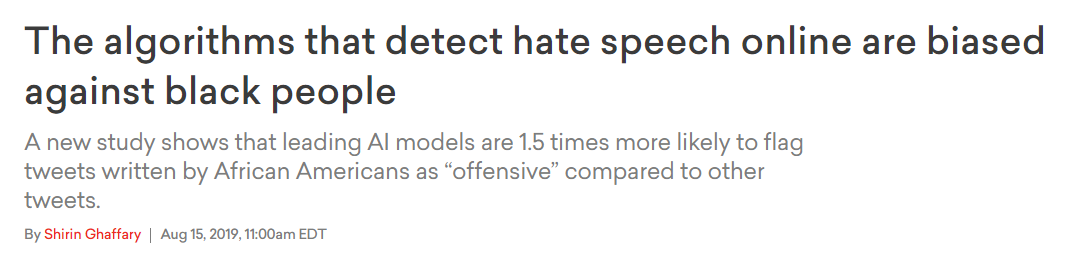
\includegraphics[width=\textwidth]{algorithmic-bias}}
    \small
    AI has limited if any true understanding → needs lots of training data to get context\\~\\

    Often AI cannot act in a fully automated way.
    \begin{itemize}
        \item Balance between sending all to humans vs only what is likely hate is a hard balance
        \item Human cost is not just a check, but exposure to potentially harmful content
    \end{itemize}
\end{frame}

\begin{frame}{Let's Talk About Training Data}
    \footnotesize
    \textbf{Data is rare in broad scope of platform}
    \begin{itemize}
        \item Enough real data for true AI models can be hard to come by
    \end{itemize}
    
    \textbf{To find training data one must either find hate as examples, or synthesize what someone may say.  This can lead to many forms of bias and blind spots:}
    \begin{itemize}
        \item Platforms, metrics, and practitioners can only see the hate they understand yet miss other types of hate
        \item Algorithmic error cases can be biased towards a certain race, ethnicity
        \item Those that build the training data as well as those doing the data mining and labeling need to be experts in hate. This expertise is hard to get without active following of hate groups.
    \end{itemize}
    
    \textbf{Language of hate evolves}
    \begin{itemize}
        \item Training data built today may not be useful in a few months as language and phrases change
    \end{itemize}
\end{frame}

\begin{frame}{}
    \begin{columns}
        \column{0.6\textwidth}
            \centering
            
\includegraphics[width=\textwidth]{newsweek}
            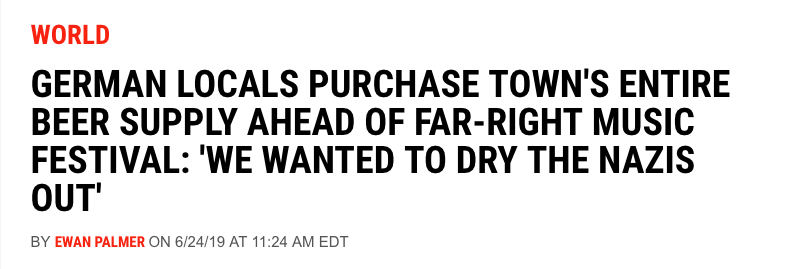
\includegraphics[width=\textwidth]{newsweek-article}
        \column{0.4\textwidth}
            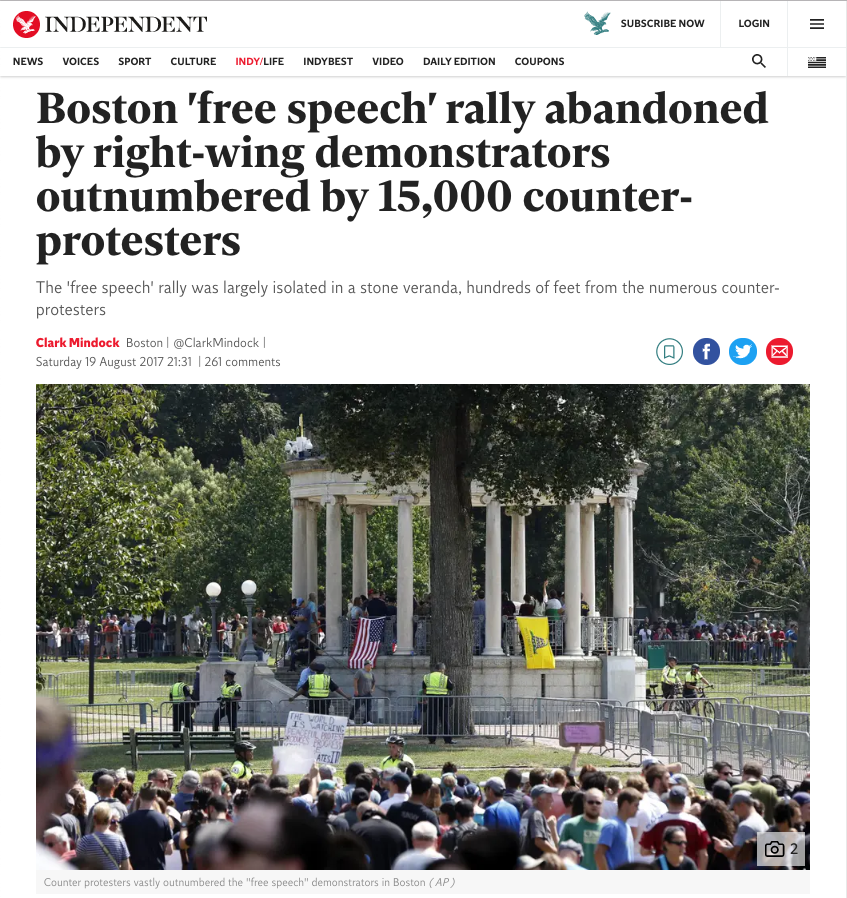
\includegraphics[width=\textwidth]{rally-abandoned-counterprotests}
    \end{columns}
\end{frame}

\begin{frame}{}
    \begin{columns}
        \column{0.55\textwidth}
            \centering
            
\includegraphics[width=\textwidth]{newsweek}
            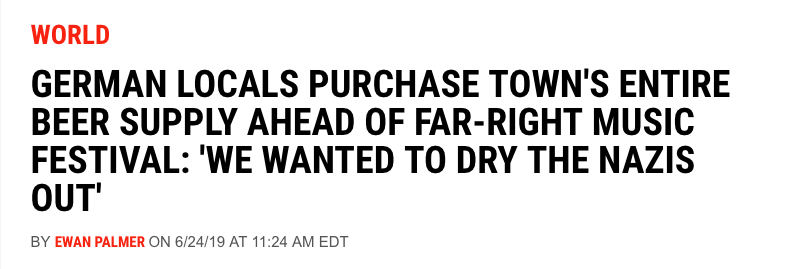
\includegraphics[width=\textwidth]{newsweek-article}
            \href{https://youtu.be/Rs4P1kKK-5k}{
\includegraphics[width=0.8\textwidth]{kkk-marchers-video}}
        \column{0.45\textwidth}
            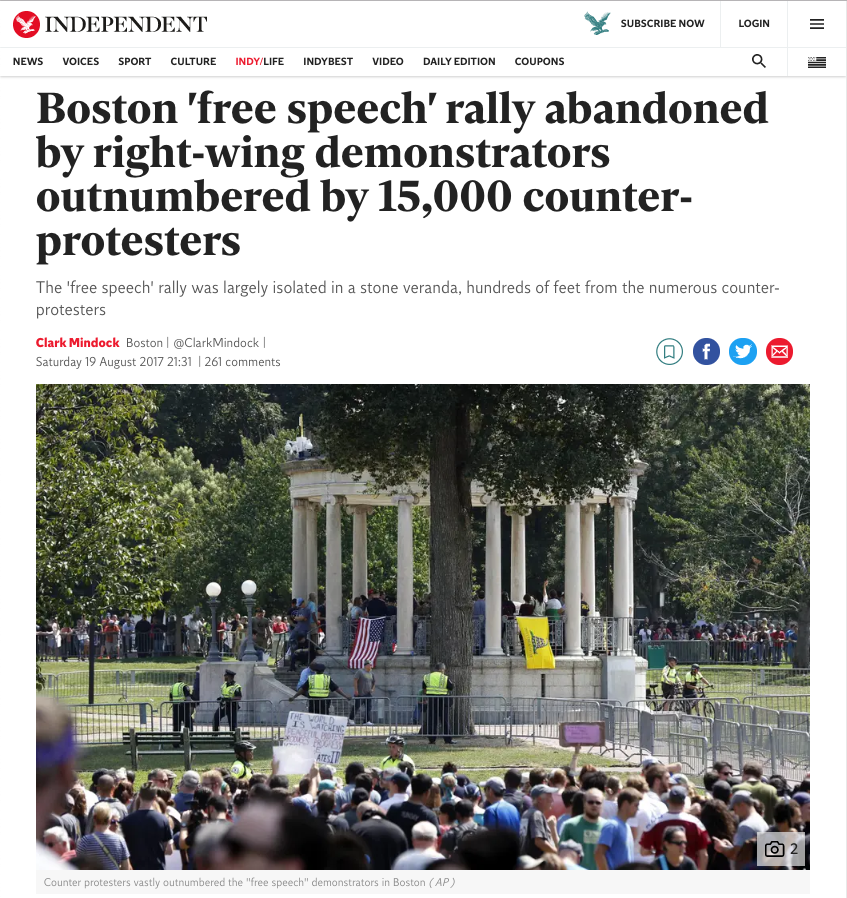
\includegraphics[width=\textwidth]{rally-abandoned-counterprotests}
    \end{columns}
\end{frame}

\begin{frame}{}
    \thispagestyle{empty}
    \AddToShipoutPictureBG*{\adjincludegraphics[trim={0 0 0 {0.52\height}}, clip, width=\paperwidth]{counterspeech}}
\end{frame}

\begin{frame}{Final thought: Is There Academic Merit to Preserving This Info?}
    \begin{columns}
        \column{0.6\textwidth}
            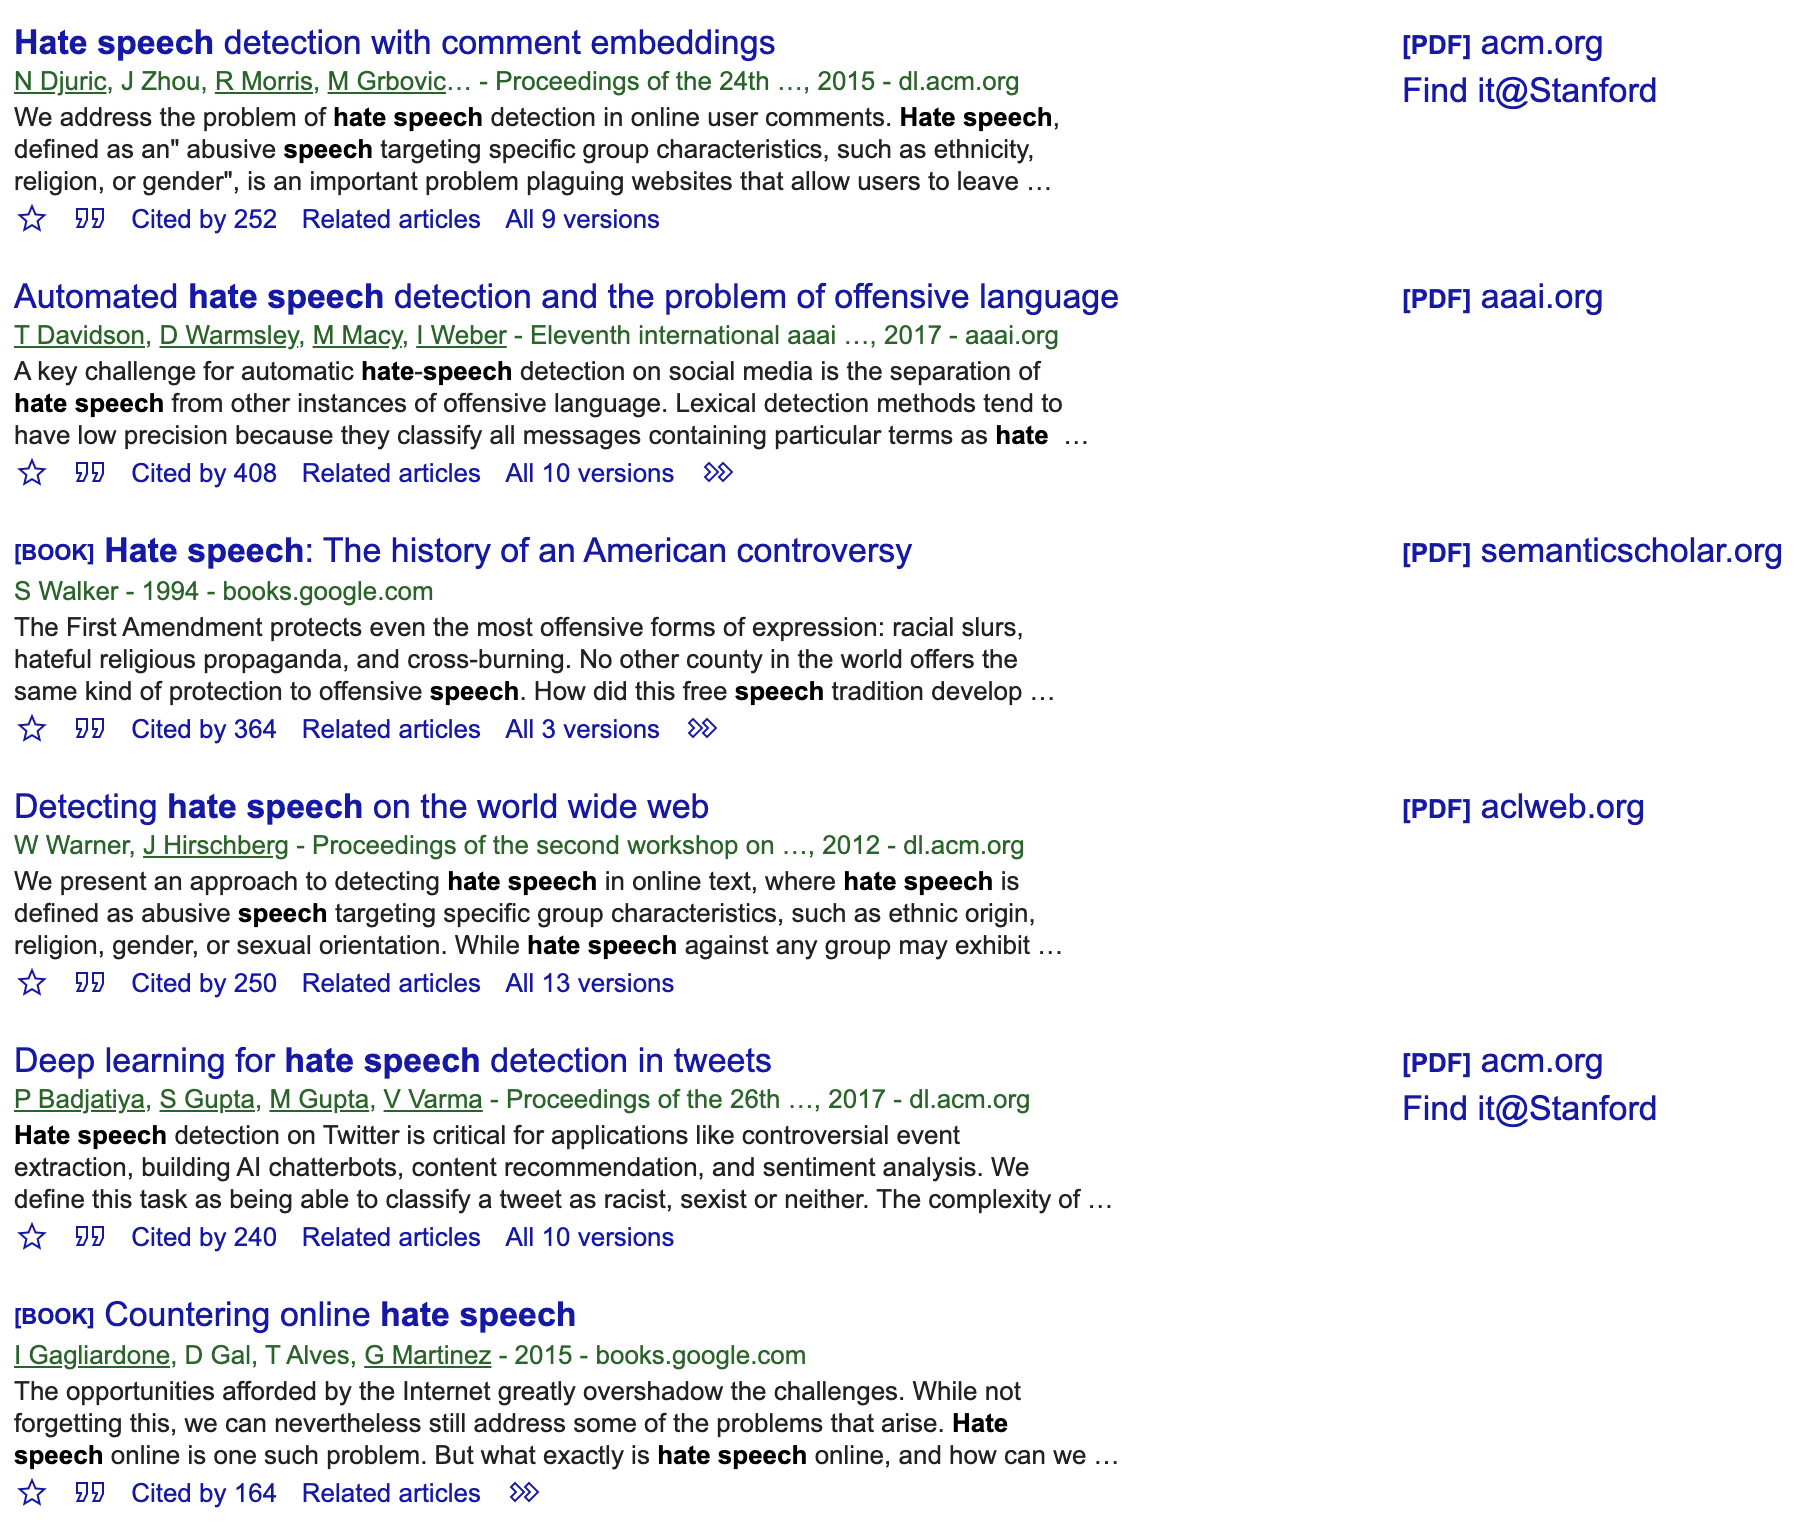
\includegraphics[width=\textwidth]{hate-speech-research}
        \column{0.3\textwidth}
            \small
            How can researchers stop the spread of something they can’t see?\\~\\
            
            What can/should the limitations be on research materials?\\~\\
            
            What is the role of companies in this dynamic?
    \end{columns}
\end{frame}

\section{Discussion}

\end{document}